% Options for packages loaded elsewhere
\PassOptionsToPackage{unicode}{hyperref}
\PassOptionsToPackage{hyphens}{url}
\PassOptionsToPackage{dvipsnames,svgnames,x11names}{xcolor}
%
\documentclass[
  letterpaper,
  DIV=11,
  numbers=noendperiod]{scrreprt}

\usepackage{amsmath,amssymb}
\usepackage{iftex}
\ifPDFTeX
  \usepackage[T1]{fontenc}
  \usepackage[utf8]{inputenc}
  \usepackage{textcomp} % provide euro and other symbols
\else % if luatex or xetex
  \usepackage{unicode-math}
  \defaultfontfeatures{Scale=MatchLowercase}
  \defaultfontfeatures[\rmfamily]{Ligatures=TeX,Scale=1}
\fi
\usepackage{lmodern}
\ifPDFTeX\else  
    % xetex/luatex font selection
\fi
% Use upquote if available, for straight quotes in verbatim environments
\IfFileExists{upquote.sty}{\usepackage{upquote}}{}
\IfFileExists{microtype.sty}{% use microtype if available
  \usepackage[]{microtype}
  \UseMicrotypeSet[protrusion]{basicmath} % disable protrusion for tt fonts
}{}
\makeatletter
\@ifundefined{KOMAClassName}{% if non-KOMA class
  \IfFileExists{parskip.sty}{%
    \usepackage{parskip}
  }{% else
    \setlength{\parindent}{0pt}
    \setlength{\parskip}{6pt plus 2pt minus 1pt}}
}{% if KOMA class
  \KOMAoptions{parskip=half}}
\makeatother
\usepackage{xcolor}
\setlength{\emergencystretch}{3em} % prevent overfull lines
\setcounter{secnumdepth}{5}
% Make \paragraph and \subparagraph free-standing
\ifx\paragraph\undefined\else
  \let\oldparagraph\paragraph
  \renewcommand{\paragraph}[1]{\oldparagraph{#1}\mbox{}}
\fi
\ifx\subparagraph\undefined\else
  \let\oldsubparagraph\subparagraph
  \renewcommand{\subparagraph}[1]{\oldsubparagraph{#1}\mbox{}}
\fi

\usepackage{color}
\usepackage{fancyvrb}
\newcommand{\VerbBar}{|}
\newcommand{\VERB}{\Verb[commandchars=\\\{\}]}
\DefineVerbatimEnvironment{Highlighting}{Verbatim}{commandchars=\\\{\}}
% Add ',fontsize=\small' for more characters per line
\usepackage{framed}
\definecolor{shadecolor}{RGB}{241,243,245}
\newenvironment{Shaded}{\begin{snugshade}}{\end{snugshade}}
\newcommand{\AlertTok}[1]{\textcolor[rgb]{0.68,0.00,0.00}{#1}}
\newcommand{\AnnotationTok}[1]{\textcolor[rgb]{0.37,0.37,0.37}{#1}}
\newcommand{\AttributeTok}[1]{\textcolor[rgb]{0.40,0.45,0.13}{#1}}
\newcommand{\BaseNTok}[1]{\textcolor[rgb]{0.68,0.00,0.00}{#1}}
\newcommand{\BuiltInTok}[1]{\textcolor[rgb]{0.00,0.23,0.31}{#1}}
\newcommand{\CharTok}[1]{\textcolor[rgb]{0.13,0.47,0.30}{#1}}
\newcommand{\CommentTok}[1]{\textcolor[rgb]{0.37,0.37,0.37}{#1}}
\newcommand{\CommentVarTok}[1]{\textcolor[rgb]{0.37,0.37,0.37}{\textit{#1}}}
\newcommand{\ConstantTok}[1]{\textcolor[rgb]{0.56,0.35,0.01}{#1}}
\newcommand{\ControlFlowTok}[1]{\textcolor[rgb]{0.00,0.23,0.31}{#1}}
\newcommand{\DataTypeTok}[1]{\textcolor[rgb]{0.68,0.00,0.00}{#1}}
\newcommand{\DecValTok}[1]{\textcolor[rgb]{0.68,0.00,0.00}{#1}}
\newcommand{\DocumentationTok}[1]{\textcolor[rgb]{0.37,0.37,0.37}{\textit{#1}}}
\newcommand{\ErrorTok}[1]{\textcolor[rgb]{0.68,0.00,0.00}{#1}}
\newcommand{\ExtensionTok}[1]{\textcolor[rgb]{0.00,0.23,0.31}{#1}}
\newcommand{\FloatTok}[1]{\textcolor[rgb]{0.68,0.00,0.00}{#1}}
\newcommand{\FunctionTok}[1]{\textcolor[rgb]{0.28,0.35,0.67}{#1}}
\newcommand{\ImportTok}[1]{\textcolor[rgb]{0.00,0.46,0.62}{#1}}
\newcommand{\InformationTok}[1]{\textcolor[rgb]{0.37,0.37,0.37}{#1}}
\newcommand{\KeywordTok}[1]{\textcolor[rgb]{0.00,0.23,0.31}{#1}}
\newcommand{\NormalTok}[1]{\textcolor[rgb]{0.00,0.23,0.31}{#1}}
\newcommand{\OperatorTok}[1]{\textcolor[rgb]{0.37,0.37,0.37}{#1}}
\newcommand{\OtherTok}[1]{\textcolor[rgb]{0.00,0.23,0.31}{#1}}
\newcommand{\PreprocessorTok}[1]{\textcolor[rgb]{0.68,0.00,0.00}{#1}}
\newcommand{\RegionMarkerTok}[1]{\textcolor[rgb]{0.00,0.23,0.31}{#1}}
\newcommand{\SpecialCharTok}[1]{\textcolor[rgb]{0.37,0.37,0.37}{#1}}
\newcommand{\SpecialStringTok}[1]{\textcolor[rgb]{0.13,0.47,0.30}{#1}}
\newcommand{\StringTok}[1]{\textcolor[rgb]{0.13,0.47,0.30}{#1}}
\newcommand{\VariableTok}[1]{\textcolor[rgb]{0.07,0.07,0.07}{#1}}
\newcommand{\VerbatimStringTok}[1]{\textcolor[rgb]{0.13,0.47,0.30}{#1}}
\newcommand{\WarningTok}[1]{\textcolor[rgb]{0.37,0.37,0.37}{\textit{#1}}}

\providecommand{\tightlist}{%
  \setlength{\itemsep}{0pt}\setlength{\parskip}{0pt}}\usepackage{longtable,booktabs,array}
\usepackage{calc} % for calculating minipage widths
% Correct order of tables after \paragraph or \subparagraph
\usepackage{etoolbox}
\makeatletter
\patchcmd\longtable{\par}{\if@noskipsec\mbox{}\fi\par}{}{}
\makeatother
% Allow footnotes in longtable head/foot
\IfFileExists{footnotehyper.sty}{\usepackage{footnotehyper}}{\usepackage{footnote}}
\makesavenoteenv{longtable}
\usepackage{graphicx}
\makeatletter
\def\maxwidth{\ifdim\Gin@nat@width>\linewidth\linewidth\else\Gin@nat@width\fi}
\def\maxheight{\ifdim\Gin@nat@height>\textheight\textheight\else\Gin@nat@height\fi}
\makeatother
% Scale images if necessary, so that they will not overflow the page
% margins by default, and it is still possible to overwrite the defaults
% using explicit options in \includegraphics[width, height, ...]{}
\setkeys{Gin}{width=\maxwidth,height=\maxheight,keepaspectratio}
% Set default figure placement to htbp
\makeatletter
\def\fps@figure{htbp}
\makeatother
\newlength{\cslhangindent}
\setlength{\cslhangindent}{1.5em}
\newlength{\csllabelwidth}
\setlength{\csllabelwidth}{3em}
\newlength{\cslentryspacingunit} % times entry-spacing
\setlength{\cslentryspacingunit}{\parskip}
\newenvironment{CSLReferences}[2] % #1 hanging-ident, #2 entry spacing
 {% don't indent paragraphs
  \setlength{\parindent}{0pt}
  % turn on hanging indent if param 1 is 1
  \ifodd #1
  \let\oldpar\par
  \def\par{\hangindent=\cslhangindent\oldpar}
  \fi
  % set entry spacing
  \setlength{\parskip}{#2\cslentryspacingunit}
 }%
 {}
\usepackage{calc}
\newcommand{\CSLBlock}[1]{#1\hfill\break}
\newcommand{\CSLLeftMargin}[1]{\parbox[t]{\csllabelwidth}{#1}}
\newcommand{\CSLRightInline}[1]{\parbox[t]{\linewidth - \csllabelwidth}{#1}\break}
\newcommand{\CSLIndent}[1]{\hspace{\cslhangindent}#1}

\usepackage{booktabs}
\usepackage{longtable}
\usepackage{array}
\usepackage{multirow}
\usepackage{wrapfig}
\usepackage{float}
\usepackage{colortbl}
\usepackage{pdflscape}
\usepackage{tabu}
\usepackage{threeparttable}
\usepackage{threeparttablex}
\usepackage[normalem]{ulem}
\usepackage{makecell}
\usepackage{xcolor}
\KOMAoption{captions}{tableheading}
\makeatletter
\makeatother
\makeatletter
\@ifpackageloaded{bookmark}{}{\usepackage{bookmark}}
\makeatother
\makeatletter
\@ifpackageloaded{caption}{}{\usepackage{caption}}
\AtBeginDocument{%
\ifdefined\contentsname
  \renewcommand*\contentsname{Table of contents}
\else
  \newcommand\contentsname{Table of contents}
\fi
\ifdefined\listfigurename
  \renewcommand*\listfigurename{List of Figures}
\else
  \newcommand\listfigurename{List of Figures}
\fi
\ifdefined\listtablename
  \renewcommand*\listtablename{List of Tables}
\else
  \newcommand\listtablename{List of Tables}
\fi
\ifdefined\figurename
  \renewcommand*\figurename{Figure}
\else
  \newcommand\figurename{Figure}
\fi
\ifdefined\tablename
  \renewcommand*\tablename{Table}
\else
  \newcommand\tablename{Table}
\fi
}
\@ifpackageloaded{float}{}{\usepackage{float}}
\floatstyle{ruled}
\@ifundefined{c@chapter}{\newfloat{codelisting}{h}{lop}}{\newfloat{codelisting}{h}{lop}[chapter]}
\floatname{codelisting}{Listing}
\newcommand*\listoflistings{\listof{codelisting}{List of Listings}}
\makeatother
\makeatletter
\@ifpackageloaded{caption}{}{\usepackage{caption}}
\@ifpackageloaded{subcaption}{}{\usepackage{subcaption}}
\makeatother
\makeatletter
\@ifpackageloaded{tcolorbox}{}{\usepackage[skins,breakable]{tcolorbox}}
\makeatother
\makeatletter
\@ifundefined{shadecolor}{\definecolor{shadecolor}{rgb}{.97, .97, .97}}
\makeatother
\makeatletter
\makeatother
\makeatletter
\makeatother
\ifLuaTeX
  \usepackage{selnolig}  % disable illegal ligatures
\fi
\IfFileExists{bookmark.sty}{\usepackage{bookmark}}{\usepackage{hyperref}}
\IfFileExists{xurl.sty}{\usepackage{xurl}}{} % add URL line breaks if available
\urlstyle{same} % disable monospaced font for URLs
\hypersetup{
  pdftitle={Programming and Data Analysis with R},
  pdfauthor={Thiyanga S. Talagala},
  colorlinks=true,
  linkcolor={blue},
  filecolor={Maroon},
  citecolor={Blue},
  urlcolor={Blue},
  pdfcreator={LaTeX via pandoc}}

\title{Programming and Data Analysis with R}
\author{Thiyanga S. Talagala}
\date{}

\begin{document}
\maketitle
\ifdefined\Shaded\renewenvironment{Shaded}{\begin{tcolorbox}[enhanced, sharp corners, breakable, borderline west={3pt}{0pt}{shadecolor}, interior hidden, boxrule=0pt, frame hidden]}{\end{tcolorbox}}\fi

\renewcommand*\contentsname{Table of contents}
{
\hypersetup{linkcolor=}
\setcounter{tocdepth}{2}
\tableofcontents
}
\bookmarksetup{startatroot}

\hypertarget{preface}{%
\chapter*{Preface}\label{preface}}
\addcontentsline{toc}{chapter}{Preface}

\markboth{Preface}{Preface}

The goal of this book is to empower you with essential skills in R
programming for statistical computing and data analysis.

Each chapter of this book is designed to be hands-on and practical, with
explanations, illustrative examples, and exercises to reinforce your
understanding.

This book is written from Quarto.

\bookmarksetup{startatroot}

\hypertarget{introduction-to-r-and-rstudio}{%
\chapter{Introduction to R and
RStudio}\label{introduction-to-r-and-rstudio}}

\hypertarget{chapter-roadmap}{%
\section{Chapter Roadmap}\label{chapter-roadmap}}

\begin{enumerate}
\def\labelenumi{\arabic{enumi}.}
\item
  What is R?
\item
  Why learn R?
\item
  R and Rstudio
\item
  Downloading R and RStudio
\item
  Installing R and RStudio
\item
  Download and Installing Rtools
\item
  Familiarize with RStudio interface
\item
  Creating and saving an RStudio project
\end{enumerate}

\hypertarget{what-is-r}{%
\section{What is R?}\label{what-is-r}}

R is a popular programming language and environment specifically
designed for statistical computing, data analysis, and data
visualisation. The language designers are \textbf{R}oss Ihaka and
\textbf{R}obert Gentleman at the Department of Statistics, University of
Auckland, New Zealand. The parent language is \textbf{S}. R is primarily
a functional programming language.

\hypertarget{why-learn-r}{%
\section{Why learn R?}\label{why-learn-r}}

\textbf{1. R is a free and open-source software package.}

\textbf{2. R is a powerful software for data analysis and statistical
computing.}

Following are some steps that need to perform for your data analysis
projects.

\begin{enumerate}
\def\labelenumi{\arabic{enumi}.}
\tightlist
\item
  Import/ Export data
\item
  Data cleaning
\item
  Data visualisation
\item
  Data modelling
\item
  Model deployment
\item
  Ensuring validity and interpretability of models
\item
  Presentation and communication of results
\end{enumerate}

Additionally, ensuring the reproducibility of data analysis and modeling
workflows is crucial for enhancing trustworthiness. R has packages to
fulfill all these data analysis and modeling needs.

\textbf{3. R can be utilized for tasks beyond traditional data analysis,
modelling and statistical computing}

\begin{enumerate}
\def\labelenumi{\arabic{enumi}.}
\item
  Scientific Writing Tools: R can be used for scientific writing,
  particularly through the use of packages like knitr rmarkdown, and
  Quarto. These packages allow you to integrate R code directly into
  documents alongside text and figures, which is highly useful for
  reproducible research and automated report generation. These are
  useful for thesis writing, book writing or any other documentation
  work. This book ``Programming and Data Analysis with R'' is written
  based on Quarto.
\item
  Website Development: R can be used developed websites, particularly
  through the use of packages like knitr rmarkdown, blogdown and Quarto.
  For example, the website https://hellor.netlify.app/ is written based
  on blogdown and https://thiyangt.github.io/rprogramming/ is written
  based on quarto.
\item
  Creating Presentations: R can generate dynamic and visually appealing
  presentations using rmarkdown, xaringan, quarto, etc. These packages
  enable you to embed R code, plots, and interactive elements directly
  into presentation slides. Here is an example presentation developed
  using xaringan https://thiyangt.github.io/whyR2021keynote/\#1
\item
  Creating Posters: R can be utilized to design scientific posters using
  packages such as posterdown. These packages provide templates for
  creating professional-looking posters directly from R Markdown
  documents. You can include plots, tables, formatted text and graphics
  in your poster design.
\item
  Web Application Development: This capability is particularly useful
  for developing data-driven tools, simulations, and dashboards that can
  be accessed through web browsers without the need for users to install
  additional software.
\end{enumerate}

\textbf{4. There is a large community of users.}

Learning a programming language with a large community of users is
particularly important for several reasons:

\begin{enumerate}
\def\labelenumi{\arabic{enumi}.}
\item
  \textbf{Support and Resources to learn:} This means there are abundant
  resources available online, including tutorials, documentation,
  forums, and open-source libraries. When you encounter issues or need
  guidance, you're more likely to find solutions quickly due to the
  active community.
\item
  \textbf{Regular updates and improvements:} Popular languages receive
  regular updates and improvements driven by community feedback and
  contributions.
\item
  \textbf{Collaboration and Career opportunities:} Since, there are many
  users you are very likely to find good job opportunities and
  collaboration opportunities.
\item
  \textbf{Networking:} Being part of a large programming community
  allows you to participate in blackthorns, and attend meetups or
  conferences. One such a R community is ``R Ladies''.
\end{enumerate}

\hypertarget{r-and-rstudio}{%
\section{R and RStudio}\label{r-and-rstudio}}

What is the difference between R and RStudio? \textbf{R is the
programming language} that provides the statistical computing
capabilities. \textbf{R Studio is an Integrated Development
Environment(IDE) for R.} \href{https://jules32.github.io/}{Dr Julia
Lowndes} illustrates the distinctions between R and RStudio using the
analogy as follows:

\begin{quote}
``If R were an airplane, RStudio would be the airport, providing many,
many supporting services that make it easier for you, the pilot, to take
off and go to awesome places. Sure, you can fly an airplane without an
airport, but having those runways and supporting infrastructure is a
game-changer.''
\end{quote}

\begin{quote}
Julie Lowndes (https://jules32.github.io/2016-07-12-Oxford/R\_RStudio/,
accessed on May 1, 2024)
\end{quote}

\hypertarget{downloading-r-and-rstudio}{%
\section{Downloading R and RStudio}\label{downloading-r-and-rstudio}}

\textbf{To download R:}

Visit the link \url{https://cran.r-project.org/} to download R. Choose
the appropriate version depending on the operating system you are using.

\textbf{To download RStudio (This can also be used to download R as
well):}

Visit the link \url{https://posit.co/download/rstudio-desktop/} to
download RStudio IDE. Make sure that you are downloading the appropriate
version that matches your computer's operating system. From the same
link you can also download the R. Furthermore, RStudio requires a
specific version of R. For example ``RStudio requires R 3.3.0+''. Make
sure you have the correct R version. The version of the R programming
language is denoted using a format like ``x.x.x'', where each ``x''
represents a number indicating the major version, minor version, and
patch level respectively.

\hypertarget{installing-r-and-rstudio}{%
\section{Installing R and Rstudio}\label{installing-r-and-rstudio}}

First, you should install R. After installation R, you can install
RStudio.

\hypertarget{installing-r}{%
\subsection{Installing R}\label{installing-r}}

Double click on the the downloaded R installer file. This will start the
install process. Usually the default options are fine. If you want to
watch a step-by-step tutorial on how to install R for Windows, you can
watch the video
\href{https://www.youtube.com/watch?v=aRwxsAEoRzs}{here}.

\hypertarget{installing-rstudio}{%
\subsection{Installing RStudio}\label{installing-rstudio}}

You must have R installed before installing RStudio. Double click on the
the downloaded RStudio installer file. This will start the install
process. Usually the default options are fine. If you want to watch a
step-by-step tutorial on how to install R for Windows, you can watch the
video \href{https://www.youtube.com/watch?v=Q1NRj2Dzdn0}{here}.

\hypertarget{download-and-installing-rtools}{%
\section{Download and Installing
Rtools}\label{download-and-installing-rtools}}

Windows users also require additional software known as Rtools,
particularly for installing certain packages. Go to the website
\url{https://cran.r-project.org/bin/windows/Rtools/} and download the
Rtools version that is compatible with your R version.

If you want to watch a step-by-step tutorial on how to install R for
Windows, you can watch the video here.

\hypertarget{familiarize-with-rstudio-interface}{%
\section{Familiarize with RStudio
interface}\label{familiarize-with-rstudio-interface}}

Step 1: Double click RStudio icon. This will open an RStudio project
window as follows:

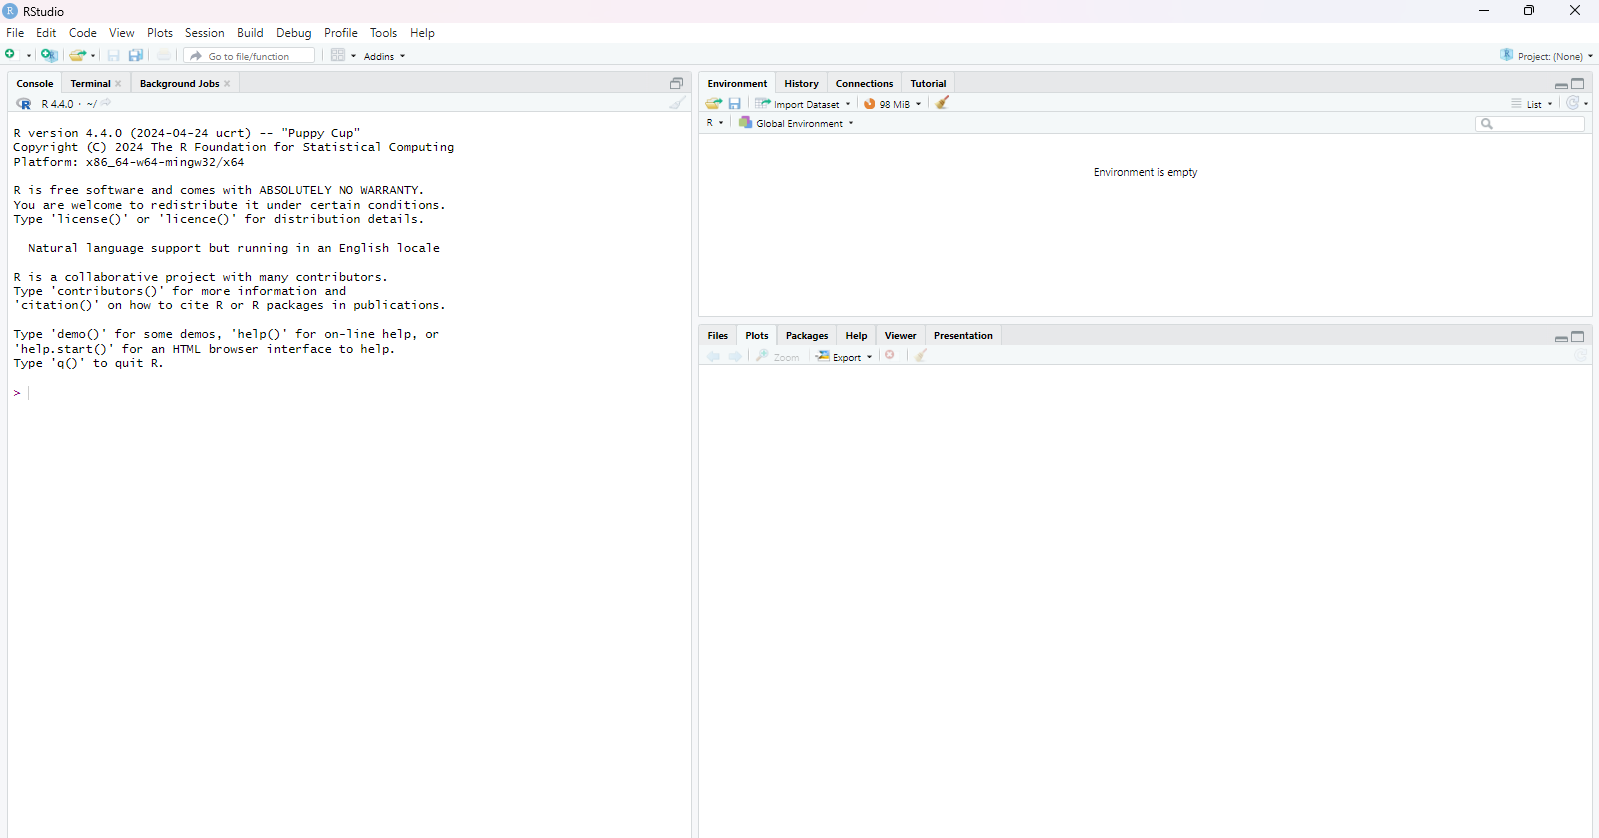
\includegraphics[width=5.33in,height=\textheight]{img/chap1/rw1.png}

Step 2: To obtain the source or script editor use the following steps:

File \textgreater{} New File \textgreater{} R Script

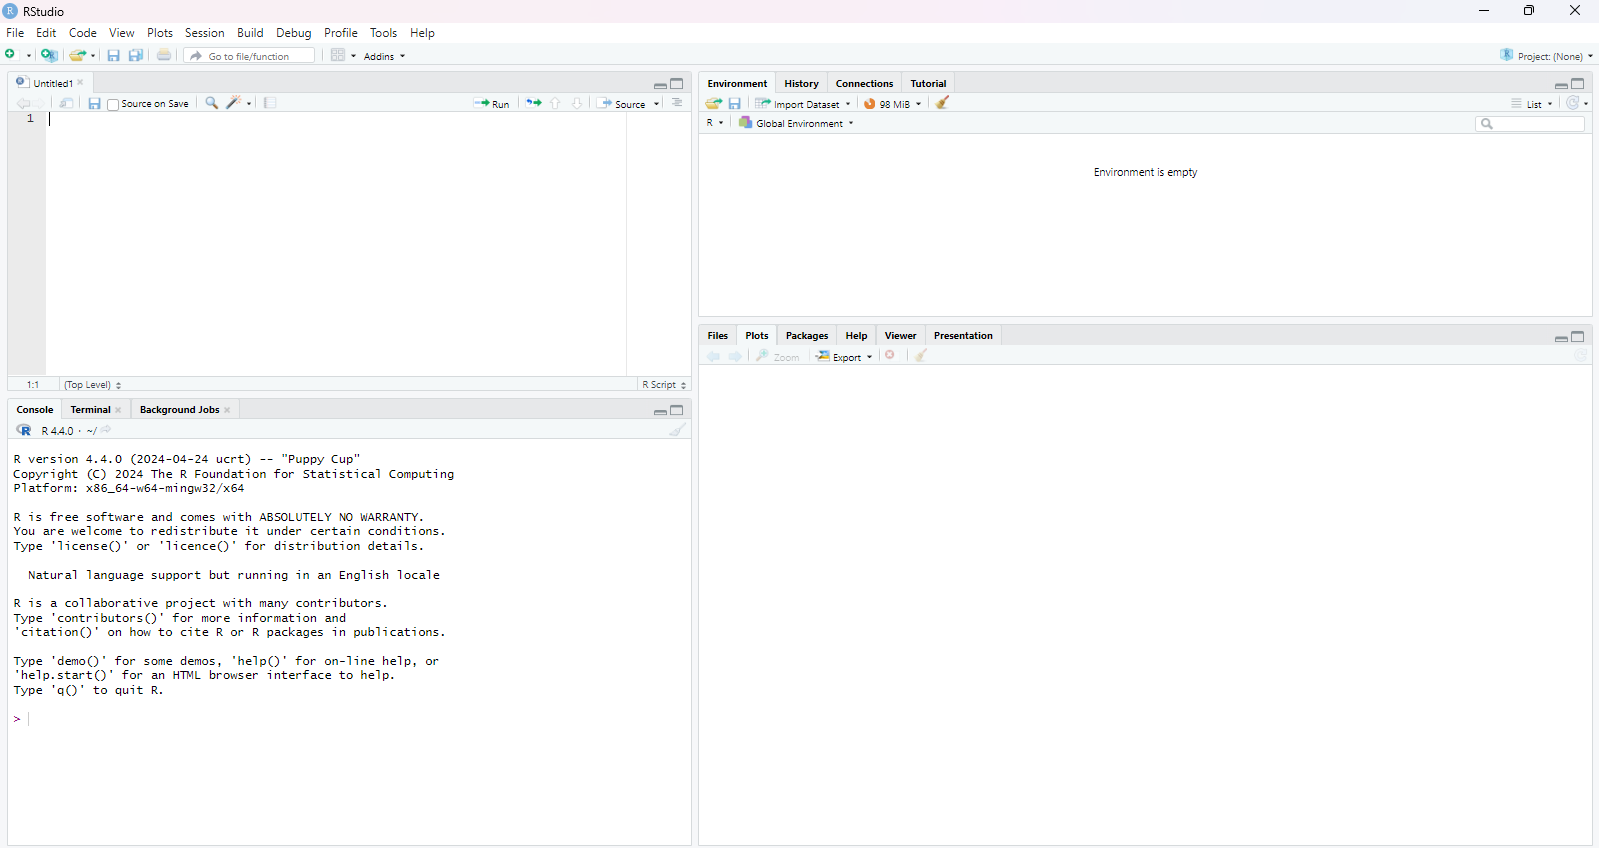
\includegraphics[width=5.33in,height=\textheight]{img/chap1/rw2.png}

Now we have four window. They are as follows:

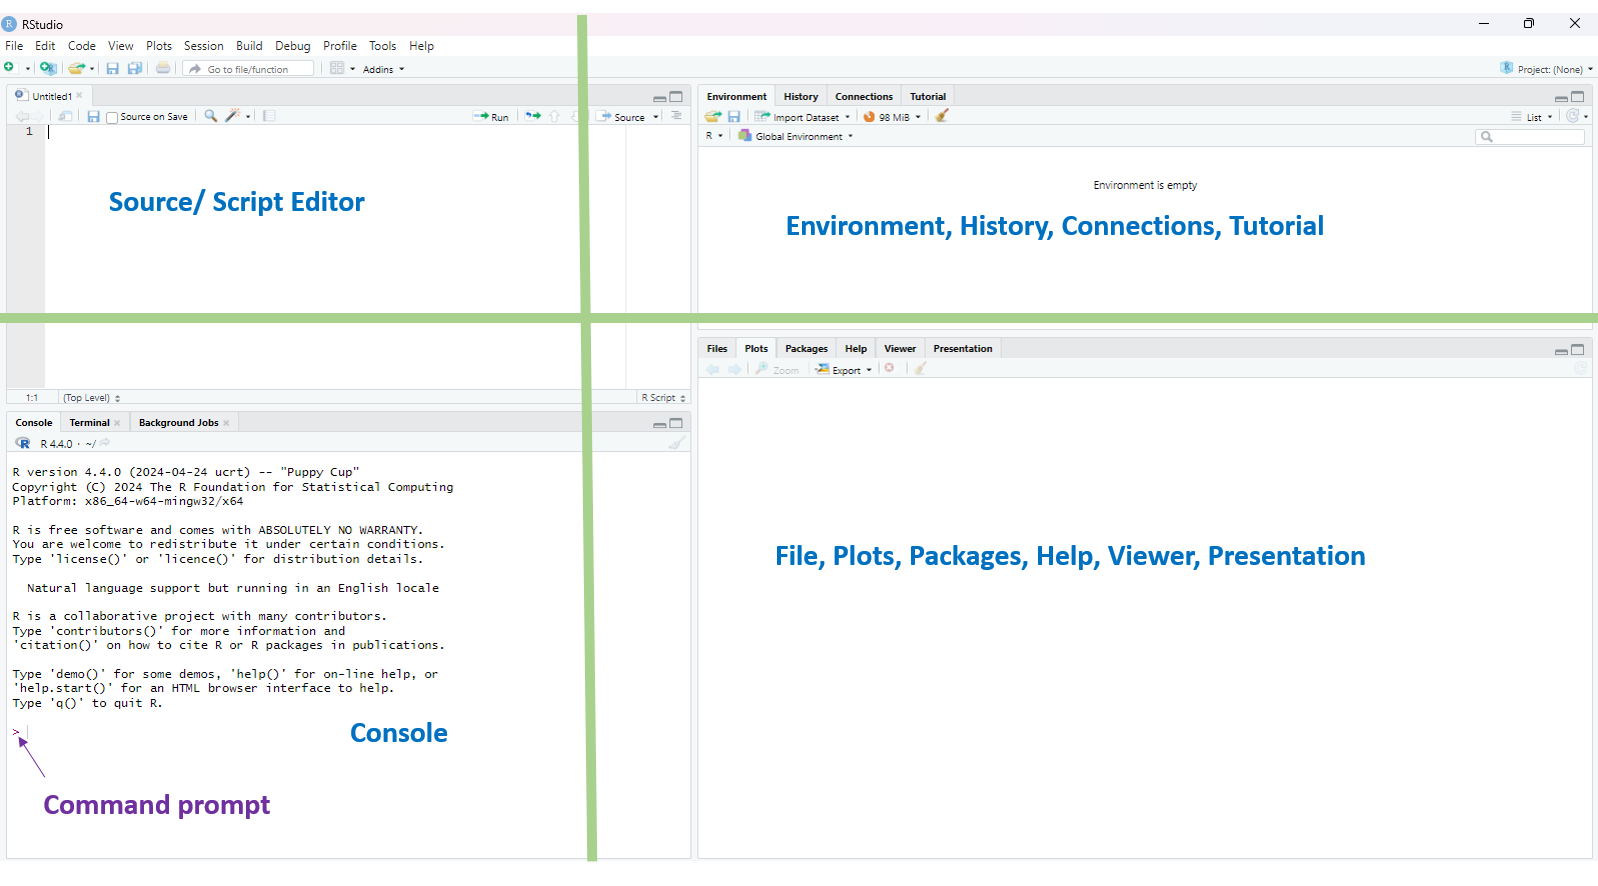
\includegraphics[width=5.33in,height=\textheight]{img/chap1/rw5.png}

\begin{enumerate}
\def\labelenumi{\arabic{enumi}.}
\tightlist
\item
  Source window: Here you can write your R codes.
\item
  Console: This is where you execute your commands to obtain the
  outputs.
\item
  Environment, History, Connections, Tutorial: Out of the different tabs
  you see here, the most important ones are the environment and the
  history tab.

  \begin{itemize}
  \item
    The Environment pane shows all the objects (like data frames,
    variables, functions, etc.) that are currently in your R session.
  \item
    The History tab keeps a record of all the commands you have run in
    the Console.
  \end{itemize}
\item
  File, Plots, Packages, Help, Viewer, Presentations:

  \begin{itemize}
  \item
    Files allows you to navigate your files.
  \item
    The graphical outputs are displayed here.
  \item
    Allows users to install, update, load, unload packages
  \item
    Help files corresponds to the functions are shown here. Help files
    provides function descriptions, examples and references for you to
    learn on your own. To access the help file of a function type ``?''
    followed by the function name . For example, `?ls`.
  \item
    Viewer/ Presentations: Useful when working with RMarkdown or Quarto
    documentations. We will look at this in Chapter 8.
  \end{itemize}
\end{enumerate}

\hypertarget{change-the-appearance-of-rstudio-pane}{%
\section{Change the appearance of RStudio
pane}\label{change-the-appearance-of-rstudio-pane}}

This is an optional step. To change the appearance, font size, RStudio
theme colour follow the steps below:

Step 1: Go to Tools \textgreater{} Global Options. You will get the
window below

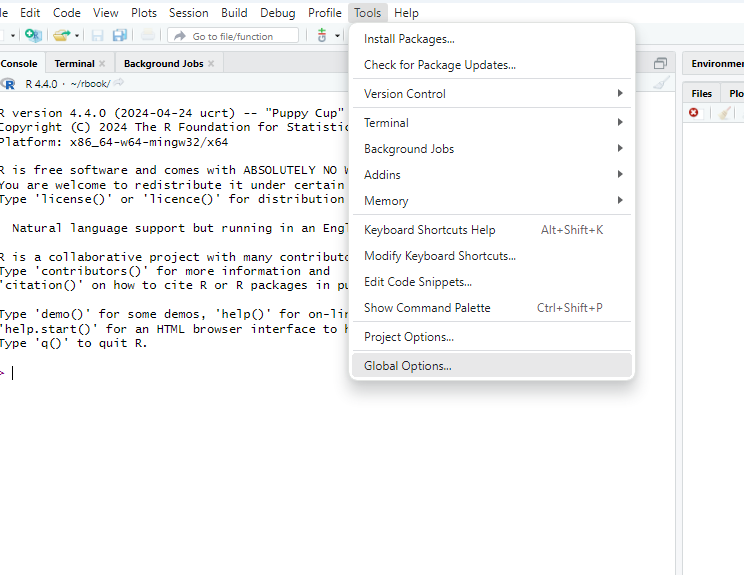
\includegraphics[width=2.48in,height=\textheight]{img/chap1/rw6.png}

Step 2: Select Appearance tab

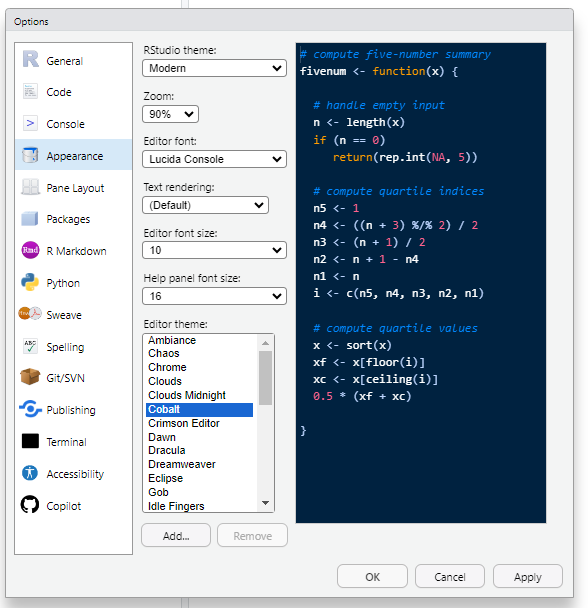
\includegraphics[width=1.96in,height=\textheight]{img/chap1/rw7.png}

Here, I select the theme to ``Cobalt''. Then the appearance of the
window will change as below:

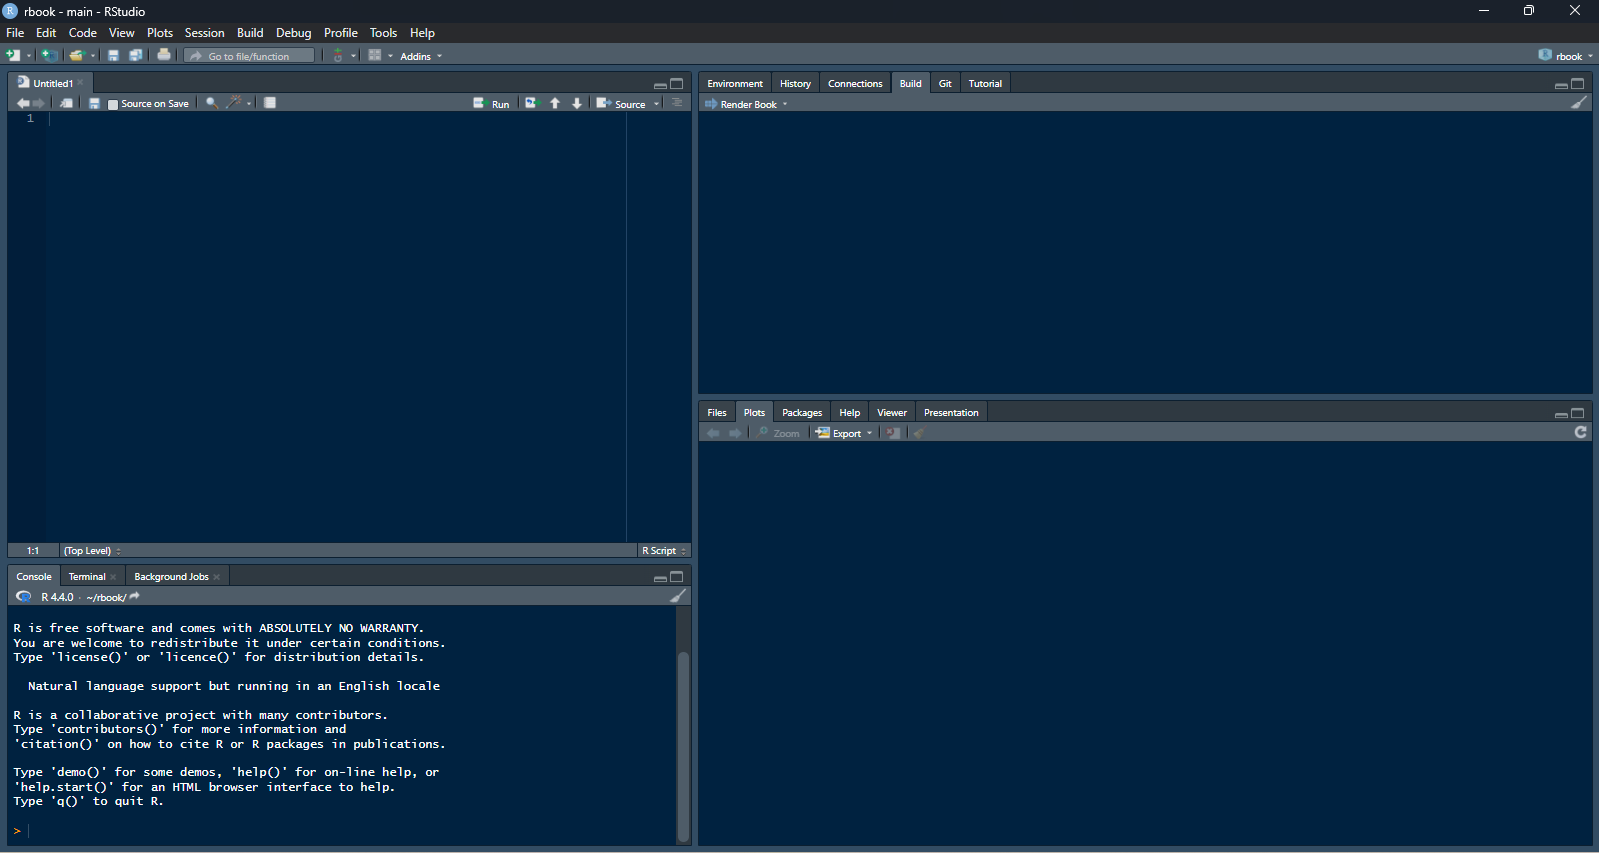
\includegraphics[width=5.33in,height=\textheight]{img/chap1/rw12.png}

\hypertarget{creating-an-rstudio-project}{%
\section{Creating an RStudio
project}\label{creating-an-rstudio-project}}

To create an RStudio project, please follow the following steps

Step 1: File \textgreater{} New Projects

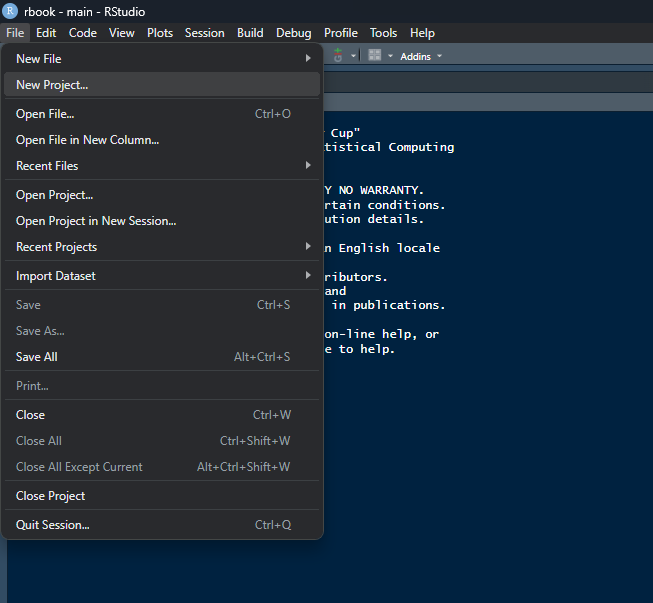
\includegraphics[width=2.18in,height=\textheight]{img/chap1/rw8.png}

Step 2: Click on the ``New Directory'' on the following window.

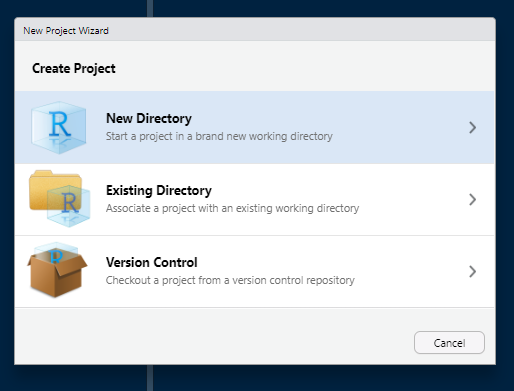
\includegraphics[width=1.71in,height=\textheight]{img/chap1/rw9.png}

Step 3: Click on ``New Project''

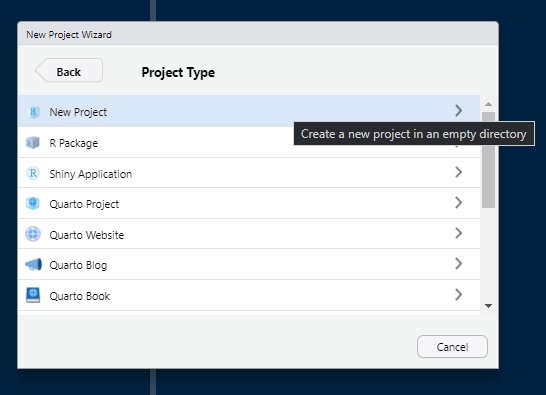
\includegraphics[width=1.82in,height=\textheight]{img/chap1/rw10.png}

Step 4: Give a directory name and a path to save

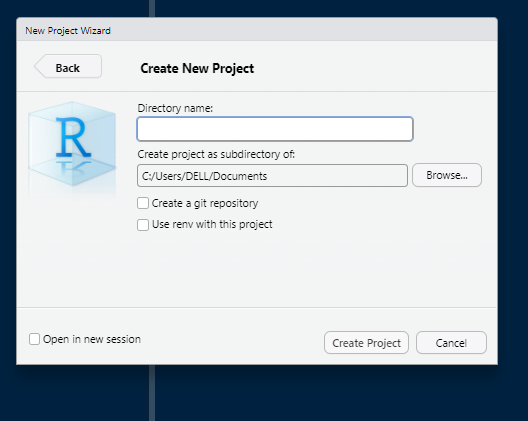
\includegraphics[width=1.76in,height=\textheight]{img/chap1/rw11.png}

\hypertarget{to-save-an-r-studio-projects}{%
\section{To save an R Studio
projects}\label{to-save-an-r-studio-projects}}

\textbf{Category 1:} If you have created a project using the steps shown
in Section 1.10, you can save your R Script files by clicking on the
floppy disk icon, as illustrated in the figure below:

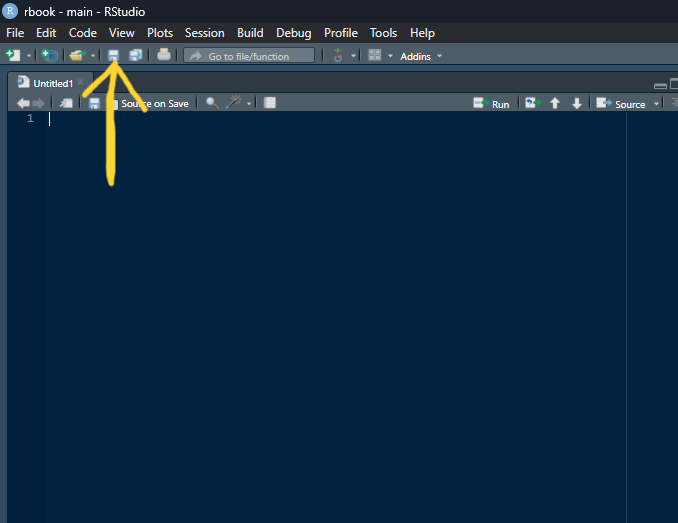
\includegraphics[width=2.26in,height=\textheight]{img/chap1/rw13.png}

\textbf{Category 2:} If you started coding without creating a project
and want to save your work, go to File \textgreater{} Save As and follow
the steps.

\hypertarget{exercise}{%
\section{Exercise}\label{exercise}}

The goal of this exercise is to help you become familiar with the R
Studio environment and create and save projects.

\begin{enumerate}
\def\labelenumi{\arabic{enumi}.}
\item
  Create a new project in the RStudio IDE. Name your project as lesson1.
\item
  Select a suitable theme for your RStudio IDE's user interface.
\end{enumerate}

\begin{quote}
Help: Navigate to Tools \textgreater{} Global Options \textgreater{}
Appearance .
\end{quote}

\begin{enumerate}
\def\labelenumi{\arabic{enumi}.}
\setcounter{enumi}{2}
\tightlist
\item
  Change the RStudio pane layout as follows:
\end{enumerate}

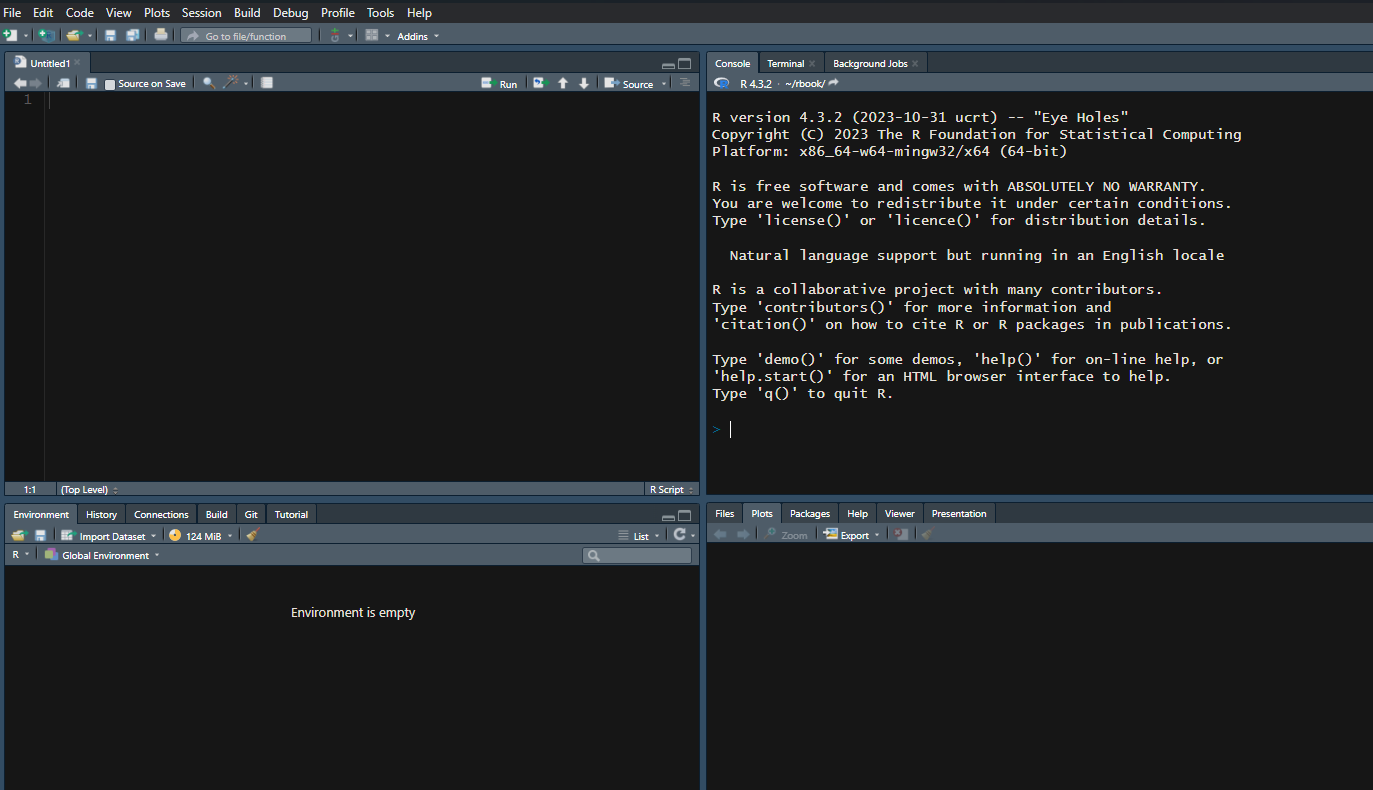
\includegraphics[width=4.58in,height=\textheight]{ch1.png}

\begin{enumerate}
\def\labelenumi{\arabic{enumi}.}
\setcounter{enumi}{3}
\item
  Create a folder called \texttt{data} inside your lesson1 project
  folder.
\item
  Create another folder called \texttt{src} inside your lesson1 project
  folder.
\item
  Open a script file and save it as \texttt{exercise1.R} inside the src
  folder.
\item
  Type the following commands on \texttt{exercise1.R} and run it on the
  console. See the changes happening under the ``Environment'' tab and
  the ``History'' tab.
\end{enumerate}

\begin{Shaded}
\begin{Highlighting}[]
\DecValTok{100} \SpecialCharTok{+} \DecValTok{200}
\FunctionTok{rnorm}\NormalTok{(}\DecValTok{100}\NormalTok{)}
\NormalTok{grades }\OtherTok{\textless{}{-}} \FunctionTok{c}\NormalTok{(}\StringTok{"A+"}\NormalTok{, }\StringTok{"A{-}"}\NormalTok{, }\StringTok{"A"}\NormalTok{, }\StringTok{"B"}\NormalTok{, }\StringTok{"F"}\NormalTok{)}
\NormalTok{random.numbers }\OtherTok{\textless{}{-}} \FunctionTok{rnorm}\NormalTok{(}\DecValTok{100}\NormalTok{)}
\NormalTok{random.numbers}\SpecialCharTok{*}\DecValTok{100}
\FunctionTok{ls}\NormalTok{()}
\end{Highlighting}
\end{Shaded}

\begin{enumerate}
\def\labelenumi{\arabic{enumi}.}
\setcounter{enumi}{7}
\item
  Close the project by saving the workspace.
\item
  Reopen your project by clicking the leason1.Rproj inside your lesson1
  folder. Open the .RData file and the .Rhistory file and observe them.
\item
  Type the following commands on exercise1.R and run them on the
  console.
\end{enumerate}

\begin{Shaded}
\begin{Highlighting}[]
\NormalTok{marks }\OtherTok{\textless{}{-}} \FunctionTok{c}\NormalTok{(}\DecValTok{100}\NormalTok{, }\DecValTok{70}\NormalTok{, }\DecValTok{80}\NormalTok{, }\DecValTok{60}\NormalTok{)}
\end{Highlighting}
\end{Shaded}

\begin{enumerate}
\def\labelenumi{\arabic{enumi}.}
\setcounter{enumi}{10}
\item
  Close the project without saving the workspace.
\item
  Reopen the lesson1.Rproj and type \texttt{ls()} on the console, and
  observe the output. (\texttt{marks} is not listed, but the other
  objects are available. Why?)
\item
  Type the following command in the console to observe changes in the
  console, environment, history, and Viewer windows. Observe the outputs
  of the code and gain an understanding of the purpose of each line.
\end{enumerate}

\begin{Shaded}
\begin{Highlighting}[]
\FunctionTok{data}\NormalTok{(}\StringTok{"iris"}\NormalTok{)}
\FunctionTok{View}\NormalTok{(iris)}
\FunctionTok{summary}\NormalTok{(iris)}
\FunctionTok{hist}\NormalTok{(iris}\SpecialCharTok{$}\NormalTok{Sepal.Length)}
\FunctionTok{plot}\NormalTok{(}\AttributeTok{x=}\NormalTok{iris}\SpecialCharTok{$}\NormalTok{Sepal.Length, }\AttributeTok{y=}\NormalTok{iris}\SpecialCharTok{$}\NormalTok{Sepal.Width) }\CommentTok{\# Method 1}
\FunctionTok{plot}\NormalTok{(Sepal.Length }\SpecialCharTok{\textasciitilde{}}\NormalTok{ Sepal.Width, }\AttributeTok{data=}\NormalTok{iris) }\CommentTok{\# Method 2}
\FunctionTok{plot}\NormalTok{(}\AttributeTok{x=}\NormalTok{iris}\SpecialCharTok{$}\NormalTok{Sepal.Length, }\AttributeTok{y=}\NormalTok{iris}\SpecialCharTok{$}\NormalTok{Sepal.Width, }\AttributeTok{col=}\NormalTok{iris}\SpecialCharTok{$}\NormalTok{Species) }
\FunctionTok{plot}\NormalTok{(Sepal.Length }\SpecialCharTok{\textasciitilde{}}\NormalTok{ Sepal.Width, }\AttributeTok{data=}\NormalTok{iris)}
\FunctionTok{plot}\NormalTok{(Sepal.Length }\SpecialCharTok{\textasciitilde{}}\NormalTok{ Sepal.Width, }\AttributeTok{pch=}\DecValTok{16}\NormalTok{, }\AttributeTok{cex=}\FloatTok{0.6}\NormalTok{, }\AttributeTok{data=}\NormalTok{iris)}
\FunctionTok{plot}\NormalTok{(Sepal.Length }\SpecialCharTok{\textasciitilde{}}\NormalTok{ Sepal.Width, }\AttributeTok{pch=}\DecValTok{16}\NormalTok{, }\AttributeTok{cex=}\FloatTok{0.6}\NormalTok{, }\AttributeTok{data=}\NormalTok{iris)}
\FunctionTok{plot}\NormalTok{(Sepal.Length }\SpecialCharTok{\textasciitilde{}}\NormalTok{ Sepal.Width, }\AttributeTok{col=}\StringTok{"forestgreen"}\NormalTok{, }\AttributeTok{pch=}\DecValTok{16}\NormalTok{, }\AttributeTok{cex=}\FloatTok{0.6}\NormalTok{, }\AttributeTok{data=}\NormalTok{iris)}
\end{Highlighting}
\end{Shaded}

\begin{enumerate}
\def\labelenumi{\arabic{enumi}.}
\setcounter{enumi}{13}
\tightlist
\item
  Type the following code to obtain list of predefined colours.
\end{enumerate}

\begin{Shaded}
\begin{Highlighting}[]
\FunctionTok{colours}\NormalTok{()}
\end{Highlighting}
\end{Shaded}

\begin{enumerate}
\def\labelenumi{\arabic{enumi}.}
\setcounter{enumi}{14}
\tightlist
\item
  Explore what changes the following code do on the last plot that you
  took.
\end{enumerate}

code chunk 15.1

\begin{Shaded}
\begin{Highlighting}[]
\FunctionTok{plot}\NormalTok{(Sepal.Length }\SpecialCharTok{\textasciitilde{}}\NormalTok{ Sepal.Width, }\AttributeTok{col=}\StringTok{"forestgreen"}\NormalTok{, }\AttributeTok{pch=}\DecValTok{16}\NormalTok{, }\AttributeTok{cex=}\FloatTok{0.6}\NormalTok{, }\AttributeTok{data=}\NormalTok{iris, }\AttributeTok{main =} \StringTok{"Scatterplot Between Sepal Length and Petal Length"}\NormalTok{,}
     \AttributeTok{xlab =} \StringTok{"Sepal Length (cm)"}\NormalTok{,}
     \AttributeTok{ylab =} \StringTok{"Sepal Width (cm)"}\NormalTok{)}
\end{Highlighting}
\end{Shaded}

code chunk 15.2

\begin{Shaded}
\begin{Highlighting}[]
\NormalTok{model }\OtherTok{\textless{}{-}} \FunctionTok{lm}\NormalTok{(Sepal.Length }\SpecialCharTok{\textasciitilde{}}\NormalTok{ Sepal.Width, }\AttributeTok{data=}\NormalTok{iris)}
\FunctionTok{plot}\NormalTok{(Sepal.Length }\SpecialCharTok{\textasciitilde{}}\NormalTok{ Sepal.Width, }\AttributeTok{col=}\StringTok{"forestgreen"}\NormalTok{, }\AttributeTok{pch=}\DecValTok{16}\NormalTok{, }\AttributeTok{cex=}\FloatTok{0.6}\NormalTok{, }\AttributeTok{data=}\NormalTok{iris, }\AttributeTok{main =} \StringTok{"Scatterplot Between Sepal Length and Petal Length"}\NormalTok{,}
     \AttributeTok{xlab =} \StringTok{"Sepal Length (cm)"}\NormalTok{,}
     \AttributeTok{ylab =} \StringTok{"Sepal Width (cm)"}\NormalTok{)}
\FunctionTok{abline}\NormalTok{(model, }\AttributeTok{col=}\StringTok{"tomato1"}\NormalTok{)}
\end{Highlighting}
\end{Shaded}

\begin{enumerate}
\def\labelenumi{\arabic{enumi}.}
\setcounter{enumi}{15}
\tightlist
\item
  Type the following commands and understand what each line of code is
  doing. Interpret the outputs.
\end{enumerate}

code chunk 16.1

\begin{Shaded}
\begin{Highlighting}[]
\FunctionTok{plot}\NormalTok{(iris)}
\end{Highlighting}
\end{Shaded}

code chunk 16.2

\begin{Shaded}
\begin{Highlighting}[]
\FunctionTok{plot}\NormalTok{(}\SpecialCharTok{\textasciitilde{}}\NormalTok{ Petal.Length }\SpecialCharTok{+}\NormalTok{ Petal.Width }\SpecialCharTok{+}\NormalTok{ Sepal.Width, }\AttributeTok{data=}\NormalTok{iris)}
\end{Highlighting}
\end{Shaded}

\begin{enumerate}
\def\labelenumi{\arabic{enumi}.}
\setcounter{enumi}{16}
\tightlist
\item
  Type the following command and open your data folder and see the
  changes that had occurred.
\end{enumerate}

\begin{Shaded}
\begin{Highlighting}[]
\FunctionTok{write.csv}\NormalTok{(iris, }\AttributeTok{file=}\StringTok{"data/iris.csv"}\NormalTok{)}
\end{Highlighting}
\end{Shaded}

\bookmarksetup{startatroot}

\hypertarget{data-structures}{%
\chapter{Data Structures}\label{data-structures}}

There are five main data structures in R. They are:

\begin{enumerate}
\def\labelenumi{\arabic{enumi}.}
\item
  vectors
\item
  matrix
\item
  array
\item
  data frame
\item
  list
\end{enumerate}

\hypertarget{vectors}{%
\section{Vectors}\label{vectors}}

\begin{enumerate}
\def\labelenumi{\arabic{enumi}.}
\item
  One dimensional data object.
\item
  Homogeneous data structure. That means data in a vector must only be
  one type or mode (numeric, character, or logical). You cannot mix
  different types of data. If you try to mix different types of data, R
  will automatically convert them into one type.
\end{enumerate}

\hypertarget{creating-vectors}{%
\section{Creating Vectors}\label{creating-vectors}}

Vectors can be made in four primary ways. They are

\begin{enumerate}
\def\labelenumi{\roman{enumi}.}
\item
  using \texttt{c()} function
\item
  using \texttt{:} function
\item
  using \texttt{seq} function
\item
  using \texttt{rep} function
\end{enumerate}

Methods ii--iv simplify vector creation. They are useful when there is a
pattern in data.

\hypertarget{concatenate-c}{%
\subsection{\texorpdfstring{Concatenate:
\texttt{c()}}{Concatenate: c()}}\label{concatenate-c}}

syntax:

Example:

The following will create the vector but not assigned a name.

\begin{Shaded}
\begin{Highlighting}[]
\FunctionTok{c}\NormalTok{(}\DecValTok{1996}\NormalTok{, }\DecValTok{1998}\NormalTok{, }\DecValTok{2000}\NormalTok{, }\DecValTok{2005}\NormalTok{)}
\end{Highlighting}
\end{Shaded}

\begin{verbatim}
[1] 1996 1998 2000 2005
\end{verbatim}

Assigning a name to vector:

The advantage of assigning a name is that we can reuse the same set of
values by calling the vector name.

\begin{Shaded}
\begin{Highlighting}[]
\NormalTok{a }\OtherTok{\textless{}{-}} \FunctionTok{c}\NormalTok{(}\DecValTok{1996}\NormalTok{, }\DecValTok{1998}\NormalTok{, }\DecValTok{2000}\NormalTok{, }\DecValTok{2005}\NormalTok{)}
\NormalTok{a}
\end{Highlighting}
\end{Shaded}

\begin{verbatim}
[1] 1996 1998 2000 2005
\end{verbatim}

\hypertarget{colon}{%
\subsection{\texorpdfstring{Colon: \texttt{:}}{Colon: :}}\label{colon}}

The \texttt{:} function can be used to create a regular decreasing or
increasing sequence.

Examples:

\begin{Shaded}
\begin{Highlighting}[]
\DecValTok{1}\SpecialCharTok{:}\DecValTok{10}
\end{Highlighting}
\end{Shaded}

\begin{verbatim}
 [1]  1  2  3  4  5  6  7  8  9 10
\end{verbatim}

\begin{Shaded}
\begin{Highlighting}[]
\DecValTok{10}\SpecialCharTok{:}\DecValTok{1}
\end{Highlighting}
\end{Shaded}

\begin{verbatim}
 [1] 10  9  8  7  6  5  4  3  2  1
\end{verbatim}

\begin{Shaded}
\begin{Highlighting}[]
\SpecialCharTok{{-}}\FloatTok{0.5}\SpecialCharTok{:}\DecValTok{10}
\end{Highlighting}
\end{Shaded}

\begin{verbatim}
 [1] -0.5  0.5  1.5  2.5  3.5  4.5  5.5  6.5  7.5  8.5  9.5
\end{verbatim}

\begin{Shaded}
\begin{Highlighting}[]
\SpecialCharTok{{-}}\FloatTok{0.3}\SpecialCharTok{:}\DecValTok{10}
\end{Highlighting}
\end{Shaded}

\begin{verbatim}
 [1] -0.3  0.7  1.7  2.7  3.7  4.7  5.7  6.7  7.7  8.7  9.7
\end{verbatim}

In all of the above sequences the increment is one. The output will
display the numbers only within the range.

\hypertarget{sequence-seq}{%
\subsection{\texorpdfstring{Sequence:
\texttt{seq}}{Sequence: seq}}\label{sequence-seq}}

\texttt{seq} function cal also be used for creating regular sequence.
With \texttt{seq} you can control the increment and length of the
output.

\textbf{Example 1}

\begin{Shaded}
\begin{Highlighting}[]
\FunctionTok{seq}\NormalTok{(}\DecValTok{1}\NormalTok{, }\DecValTok{19}\NormalTok{)}
\end{Highlighting}
\end{Shaded}

\begin{verbatim}
 [1]  1  2  3  4  5  6  7  8  9 10 11 12 13 14 15 16 17 18 19
\end{verbatim}

\textbf{Example 2}

\begin{Shaded}
\begin{Highlighting}[]
\FunctionTok{seq}\NormalTok{(}\DecValTok{1}\NormalTok{, }\DecValTok{19}\NormalTok{, }\AttributeTok{length.out=}\DecValTok{8}\NormalTok{)}
\end{Highlighting}
\end{Shaded}

\begin{verbatim}
[1]  1.000000  3.571429  6.142857  8.714286 11.285714 13.857143 16.428571
[8] 19.000000
\end{verbatim}

\textbf{Example 3}

\begin{Shaded}
\begin{Highlighting}[]
\FunctionTok{seq}\NormalTok{(}\DecValTok{1}\NormalTok{, }\DecValTok{19}\NormalTok{, }\AttributeTok{by =} \DecValTok{3}\NormalTok{)}
\end{Highlighting}
\end{Shaded}

\begin{verbatim}
[1]  1  4  7 10 13 16 19
\end{verbatim}

\hypertarget{repeat-rep}{%
\section{\texorpdfstring{Repeat:
\texttt{rep}}{Repeat: rep}}\label{repeat-rep}}

The \texttt{rep} function can be used if there is a pattern of
repetition in the data.

\textbf{Example 1}

The number 8 is repeated three times.

\begin{Shaded}
\begin{Highlighting}[]
\FunctionTok{rep}\NormalTok{(}\DecValTok{8}\NormalTok{, }\DecValTok{5}\NormalTok{)}
\end{Highlighting}
\end{Shaded}

\begin{verbatim}
[1] 8 8 8 8 8
\end{verbatim}

\textbf{Example 2}

The sequence \texttt{1,\ 2,\ 3} is repeated five times.

\begin{Shaded}
\begin{Highlighting}[]
\FunctionTok{rep}\NormalTok{(}\DecValTok{1}\SpecialCharTok{:}\DecValTok{3}\NormalTok{, }\AttributeTok{times=}\DecValTok{5}\NormalTok{)}
\end{Highlighting}
\end{Shaded}

\begin{verbatim}
 [1] 1 2 3 1 2 3 1 2 3 1 2 3 1 2 3
\end{verbatim}

\textbf{Example 3}

Same as in Example 2 above.

\begin{Shaded}
\begin{Highlighting}[]
\FunctionTok{rep}\NormalTok{(}\DecValTok{1}\SpecialCharTok{:}\DecValTok{3}\NormalTok{, }\DecValTok{5}\NormalTok{)}
\end{Highlighting}
\end{Shaded}

\begin{verbatim}
 [1] 1 2 3 1 2 3 1 2 3 1 2 3 1 2 3
\end{verbatim}

\textbf{Example 4}

Each element in the sequence is repeated five times.

\begin{Shaded}
\begin{Highlighting}[]
\FunctionTok{rep}\NormalTok{(}\DecValTok{1}\SpecialCharTok{:}\DecValTok{3}\NormalTok{, }\AttributeTok{each=}\DecValTok{5}\NormalTok{)}
\end{Highlighting}
\end{Shaded}

\begin{verbatim}
 [1] 1 1 1 1 1 2 2 2 2 2 3 3 3 3 3
\end{verbatim}

\textbf{Example 5}

First, each element is repeated five times. After that, the whole
sequence is repeated three times.

\begin{Shaded}
\begin{Highlighting}[]
\FunctionTok{rep}\NormalTok{(}\DecValTok{1}\SpecialCharTok{:}\DecValTok{3}\NormalTok{, }\AttributeTok{each=}\DecValTok{5}\NormalTok{, }\AttributeTok{times=}\DecValTok{3}\NormalTok{)}
\end{Highlighting}
\end{Shaded}

\begin{verbatim}
 [1] 1 1 1 1 1 2 2 2 2 2 3 3 3 3 3 1 1 1 1 1 2 2 2 2 2 3 3 3 3 3 1 1 1 1 1 2 2 2
[39] 2 2 3 3 3 3 3
\end{verbatim}

\textbf{Example 6}

Same as before. Changing the ordering of \texttt{each} and \texttt{time}
does not change the output.

\begin{Shaded}
\begin{Highlighting}[]
\FunctionTok{rep}\NormalTok{(}\DecValTok{1}\SpecialCharTok{:}\DecValTok{3}\NormalTok{, }\AttributeTok{times=}\DecValTok{3}\NormalTok{, }\AttributeTok{each=}\DecValTok{5}\NormalTok{)}
\end{Highlighting}
\end{Shaded}

\begin{verbatim}
 [1] 1 1 1 1 1 2 2 2 2 2 3 3 3 3 3 1 1 1 1 1 2 2 2 2 2 3 3 3 3 3 1 1 1 1 1 2 2 2
[39] 2 2 3 3 3 3 3
\end{verbatim}

\hypertarget{coercion}{%
\section{Coercion}\label{coercion}}

When you try to include different types they will be coerced to the most
flexible type.

\begin{Shaded}
\begin{Highlighting}[]
\NormalTok{a }\OtherTok{\textless{}{-}} \FunctionTok{c}\NormalTok{(}\DecValTok{1}\NormalTok{, }\DecValTok{3}\NormalTok{, }\StringTok{"GPA"}\NormalTok{, }\ConstantTok{TRUE}\NormalTok{, 1L)}
\FunctionTok{typeof}\NormalTok{(a)}
\end{Highlighting}
\end{Shaded}

\begin{verbatim}
[1] "character"
\end{verbatim}

Explicit coercion means that if we try to convert a data type to another
data type intentionally using a specific function. For example,

\begin{Shaded}
\begin{Highlighting}[]
\NormalTok{b }\OtherTok{\textless{}{-}} \FunctionTok{c}\NormalTok{(}\FloatTok{3.1}\NormalTok{, }\FloatTok{3.2}\NormalTok{, }\FloatTok{3.7}\NormalTok{, }\FloatTok{5.9}\NormalTok{)}
\NormalTok{b}
\end{Highlighting}
\end{Shaded}

\begin{verbatim}
[1] 3.1 3.2 3.7 5.9
\end{verbatim}

\begin{Shaded}
\begin{Highlighting}[]
\FunctionTok{as.integer}\NormalTok{(b)}
\end{Highlighting}
\end{Shaded}

\begin{verbatim}
[1] 3 3 3 5
\end{verbatim}

\hypertarget{functions-that-can-be-used-to-inspect-vectors}{%
\section{Functions that can be used to inspect
vectors}\label{functions-that-can-be-used-to-inspect-vectors}}

Consider the vector below

\begin{Shaded}
\begin{Highlighting}[]
\NormalTok{example.vec }\OtherTok{\textless{}{-}} \FunctionTok{c}\NormalTok{(}\DecValTok{1}\NormalTok{,  }\DecValTok{2}\NormalTok{,  }\DecValTok{3}\NormalTok{, }\DecValTok{4}\NormalTok{, }\DecValTok{5}\NormalTok{, }\DecValTok{6}\NormalTok{, }\DecValTok{7}\NormalTok{, }\DecValTok{8}\NormalTok{)}
\end{Highlighting}
\end{Shaded}

\begin{enumerate}
\def\labelenumi{\arabic{enumi}.}
\tightlist
\item
  To check the storage mode
\end{enumerate}

\begin{Shaded}
\begin{Highlighting}[]
\FunctionTok{typeof}\NormalTok{(example.vec)}
\end{Highlighting}
\end{Shaded}

\begin{verbatim}
[1] "double"
\end{verbatim}

\begin{enumerate}
\def\labelenumi{\arabic{enumi}.}
\setcounter{enumi}{1}
\tightlist
\item
  To check the class type
\end{enumerate}

\begin{Shaded}
\begin{Highlighting}[]
\FunctionTok{class}\NormalTok{(example.vec)}
\end{Highlighting}
\end{Shaded}

\begin{verbatim}
[1] "numeric"
\end{verbatim}

\begin{enumerate}
\def\labelenumi{\arabic{enumi}.}
\setcounter{enumi}{2}
\tightlist
\item
  Testing functions
\end{enumerate}

\begin{Shaded}
\begin{Highlighting}[]
\FunctionTok{is.character}\NormalTok{(example.vec)}
\end{Highlighting}
\end{Shaded}

\begin{verbatim}
[1] FALSE
\end{verbatim}

\begin{Shaded}
\begin{Highlighting}[]
\FunctionTok{is.integer}\NormalTok{(example.vec)}
\end{Highlighting}
\end{Shaded}

\begin{verbatim}
[1] FALSE
\end{verbatim}

\begin{Shaded}
\begin{Highlighting}[]
\FunctionTok{is.logical}\NormalTok{(example.vec)}
\end{Highlighting}
\end{Shaded}

\begin{verbatim}
[1] FALSE
\end{verbatim}

\begin{Shaded}
\begin{Highlighting}[]
\FunctionTok{is.double}\NormalTok{(example.vec)}
\end{Highlighting}
\end{Shaded}

\begin{verbatim}
[1] TRUE
\end{verbatim}

\begin{enumerate}
\def\labelenumi{\arabic{enumi}.}
\setcounter{enumi}{3}
\tightlist
\item
  Mathematical and statistical functions
\end{enumerate}

\begin{Shaded}
\begin{Highlighting}[]
\FunctionTok{sum}\NormalTok{(example.vec)}
\end{Highlighting}
\end{Shaded}

\begin{verbatim}
[1] 36
\end{verbatim}

\begin{Shaded}
\begin{Highlighting}[]
\FunctionTok{mean}\NormalTok{(example.vec)}
\end{Highlighting}
\end{Shaded}

\begin{verbatim}
[1] 4.5
\end{verbatim}

\begin{Shaded}
\begin{Highlighting}[]
\FunctionTok{summary}\NormalTok{(example.vec)}
\end{Highlighting}
\end{Shaded}

\begin{verbatim}
   Min. 1st Qu.  Median    Mean 3rd Qu.    Max. 
   1.00    2.75    4.50    4.50    6.25    8.00 
\end{verbatim}

\begin{enumerate}
\def\labelenumi{\arabic{enumi}.}
\setcounter{enumi}{4}
\tightlist
\item
  To check if there are any missing values
\end{enumerate}

\begin{Shaded}
\begin{Highlighting}[]
\FunctionTok{is.na}\NormalTok{(example.vec)}
\end{Highlighting}
\end{Shaded}

\begin{verbatim}
[1] FALSE FALSE FALSE FALSE FALSE FALSE FALSE FALSE
\end{verbatim}

There are many more functions that you can use with vectors. We will
learn about them in the upcoming chapters.

\hypertarget{exercise-1}{%
\section{Exercise}\label{exercise-1}}

\begin{enumerate}
\def\labelenumi{\arabic{enumi}.}
\tightlist
\item
  Write R codes to create the following vectors: If you see patterns in
  the data, use vector simplification methods.
\end{enumerate}

\begin{enumerate}
\def\labelenumi{\roman{enumi}.}
\tightlist
\item
\end{enumerate}

\begin{verbatim}
[1] 1990 1992 1934 1957 1970 2000 2005
\end{verbatim}

\begin{enumerate}
\def\labelenumi{\roman{enumi}.}
\setcounter{enumi}{1}
\tightlist
\item
\end{enumerate}

\begin{verbatim}
 [1] 3 6 9 3 6 9 3 6 9 3 6 9 3 6 9
\end{verbatim}

\begin{enumerate}
\def\labelenumi{\roman{enumi}.}
\setcounter{enumi}{2}
\tightlist
\item
\end{enumerate}

\begin{verbatim}
 [1] 3 3 3 3 3 6 6 6 6 6 9 9 9 9 9
\end{verbatim}

\begin{enumerate}
\def\labelenumi{\roman{enumi}.}
\setcounter{enumi}{3}
\tightlist
\item
\end{enumerate}

\begin{verbatim}
 [1] 3 3 3 3 3 6 6 6 6 6 9 9 9 9 9 3 3 3 3 3 6 6 6 6 6 9 9 9 9 9
\end{verbatim}

\begin{enumerate}
\def\labelenumi{\alph{enumi}.}
\setcounter{enumi}{21}
\tightlist
\item
\end{enumerate}

\begin{verbatim}
 [1]  1  4  7 10 13 16 19 22 25 28 31 34
\end{verbatim}

\begin{enumerate}
\def\labelenumi{\roman{enumi}.}
\setcounter{enumi}{5}
\tightlist
\item
\end{enumerate}

\begin{verbatim}
  [1] 0.1000000 0.1020202 0.1040404 0.1060606 0.1080808 0.1101010 0.1121212
  [8] 0.1141414 0.1161616 0.1181818 0.1202020 0.1222222 0.1242424 0.1262626
 [15] 0.1282828 0.1303030 0.1323232 0.1343434 0.1363636 0.1383838 0.1404040
 [22] 0.1424242 0.1444444 0.1464646 0.1484848 0.1505051 0.1525253 0.1545455
 [29] 0.1565657 0.1585859 0.1606061 0.1626263 0.1646465 0.1666667 0.1686869
 [36] 0.1707071 0.1727273 0.1747475 0.1767677 0.1787879 0.1808081 0.1828283
 [43] 0.1848485 0.1868687 0.1888889 0.1909091 0.1929293 0.1949495 0.1969697
 [50] 0.1989899 0.2010101 0.2030303 0.2050505 0.2070707 0.2090909 0.2111111
 [57] 0.2131313 0.2151515 0.2171717 0.2191919 0.2212121 0.2232323 0.2252525
 [64] 0.2272727 0.2292929 0.2313131 0.2333333 0.2353535 0.2373737 0.2393939
 [71] 0.2414141 0.2434343 0.2454545 0.2474747 0.2494949 0.2515152 0.2535354
 [78] 0.2555556 0.2575758 0.2595960 0.2616162 0.2636364 0.2656566 0.2676768
 [85] 0.2696970 0.2717172 0.2737374 0.2757576 0.2777778 0.2797980 0.2818182
 [92] 0.2838384 0.2858586 0.2878788 0.2898990 0.2919192 0.2939394 0.2959596
 [99] 0.2979798 0.3000000
\end{verbatim}

\begin{enumerate}
\def\labelenumi{\roman{enumi}.}
\setcounter{enumi}{6}
\tightlist
\item
\end{enumerate}

\begin{verbatim}
 [1] -0.5  0.5  1.5  2.5  3.5  4.5  5.5  6.5  7.5  8.5  9.5 10.5
\end{verbatim}

\begin{enumerate}
\def\labelenumi{\roman{enumi}.}
\setcounter{enumi}{7}
\tightlist
\item
\end{enumerate}

\begin{verbatim}
 [1]  2  4  6  8 10 12 14 16 18 20 22 24 26 28 30 32 34 36 38 40 42 44 46 48 50
[26] 52 54 56 58 60 62 64 66 68 70 72
\end{verbatim}

\begin{enumerate}
\def\labelenumi{\arabic{enumi}.}
\setcounter{enumi}{1}
\tightlist
\item
  Use the \texttt{typeof()} function to check the R storage mode of the
  following vectors and \texttt{class()} to check the class type of the
  vector.
\end{enumerate}

\begin{Shaded}
\begin{Highlighting}[]
\NormalTok{logical\_vector }\OtherTok{\textless{}{-}} \FunctionTok{c}\NormalTok{(}\ConstantTok{TRUE}\NormalTok{, }\ConstantTok{FALSE}\NormalTok{, }\ConstantTok{TRUE}\NormalTok{, }\ConstantTok{FALSE}\NormalTok{)}
\NormalTok{integer\_vector }\OtherTok{\textless{}{-}} \FunctionTok{c}\NormalTok{(1L, 2L, 3L, 4L)}
\NormalTok{double\_vector }\OtherTok{\textless{}{-}} \FunctionTok{c}\NormalTok{(}\FloatTok{1.1}\NormalTok{, }\FloatTok{2.2}\NormalTok{, }\FloatTok{3.3}\NormalTok{, }\FloatTok{4.4}\NormalTok{)}
\NormalTok{complex\_vector }\OtherTok{\textless{}{-}} \FunctionTok{c}\NormalTok{(}\DecValTok{1}\SpecialCharTok{+}\NormalTok{1i, }\DecValTok{2}\SpecialCharTok{+}\NormalTok{2i, }\DecValTok{3}\SpecialCharTok{+}\NormalTok{3i, }\DecValTok{4}\SpecialCharTok{+}\NormalTok{4i)}
\NormalTok{character\_vector }\OtherTok{\textless{}{-}} \FunctionTok{c}\NormalTok{(}\StringTok{"a"}\NormalTok{, }\StringTok{"b"}\NormalTok{, }\StringTok{"c"}\NormalTok{, }\StringTok{"d"}\NormalTok{)}
\NormalTok{null\_vector }\OtherTok{\textless{}{-}} \ConstantTok{NULL}
\NormalTok{time\_data }\OtherTok{\textless{}{-}} \DecValTok{1996}\SpecialCharTok{:}\DecValTok{2006}
\NormalTok{time\_series\_data }\OtherTok{\textless{}{-}} \FunctionTok{ts}\NormalTok{(}\DecValTok{1996}\SpecialCharTok{:}\DecValTok{2006}\NormalTok{)}
\end{Highlighting}
\end{Shaded}

\begin{enumerate}
\def\labelenumi{\arabic{enumi}.}
\setcounter{enumi}{2}
\item
  Create the vector (3, 3, 3, . . . 3, 6, 6, . . . 6, 9, 9, 9, . . . 9),
  where there are 10 occurrences of 3, 20 occurrences of 6 and 30
  occurrences of 9.
\item
  Find the value of the following expression.
\end{enumerate}

\begin{enumerate}
\def\labelenumi{\roman{enumi}.}
\item
  \(\sum_{i=1}^{100}i\)
\item
  \(\sum_{i=1}^{100}i^2\)
\end{enumerate}

\begin{enumerate}
\def\labelenumi{\arabic{enumi}.}
\setcounter{enumi}{4}
\item
  Generate a sequence using the code seq(from=1, to=10, by=1). What
  other ways can you generate the same sequence?
\item
  Create a vector to hold population values, and label each element with
  the corresponding province name. The plot will display population
  values when hovered over.
\end{enumerate}

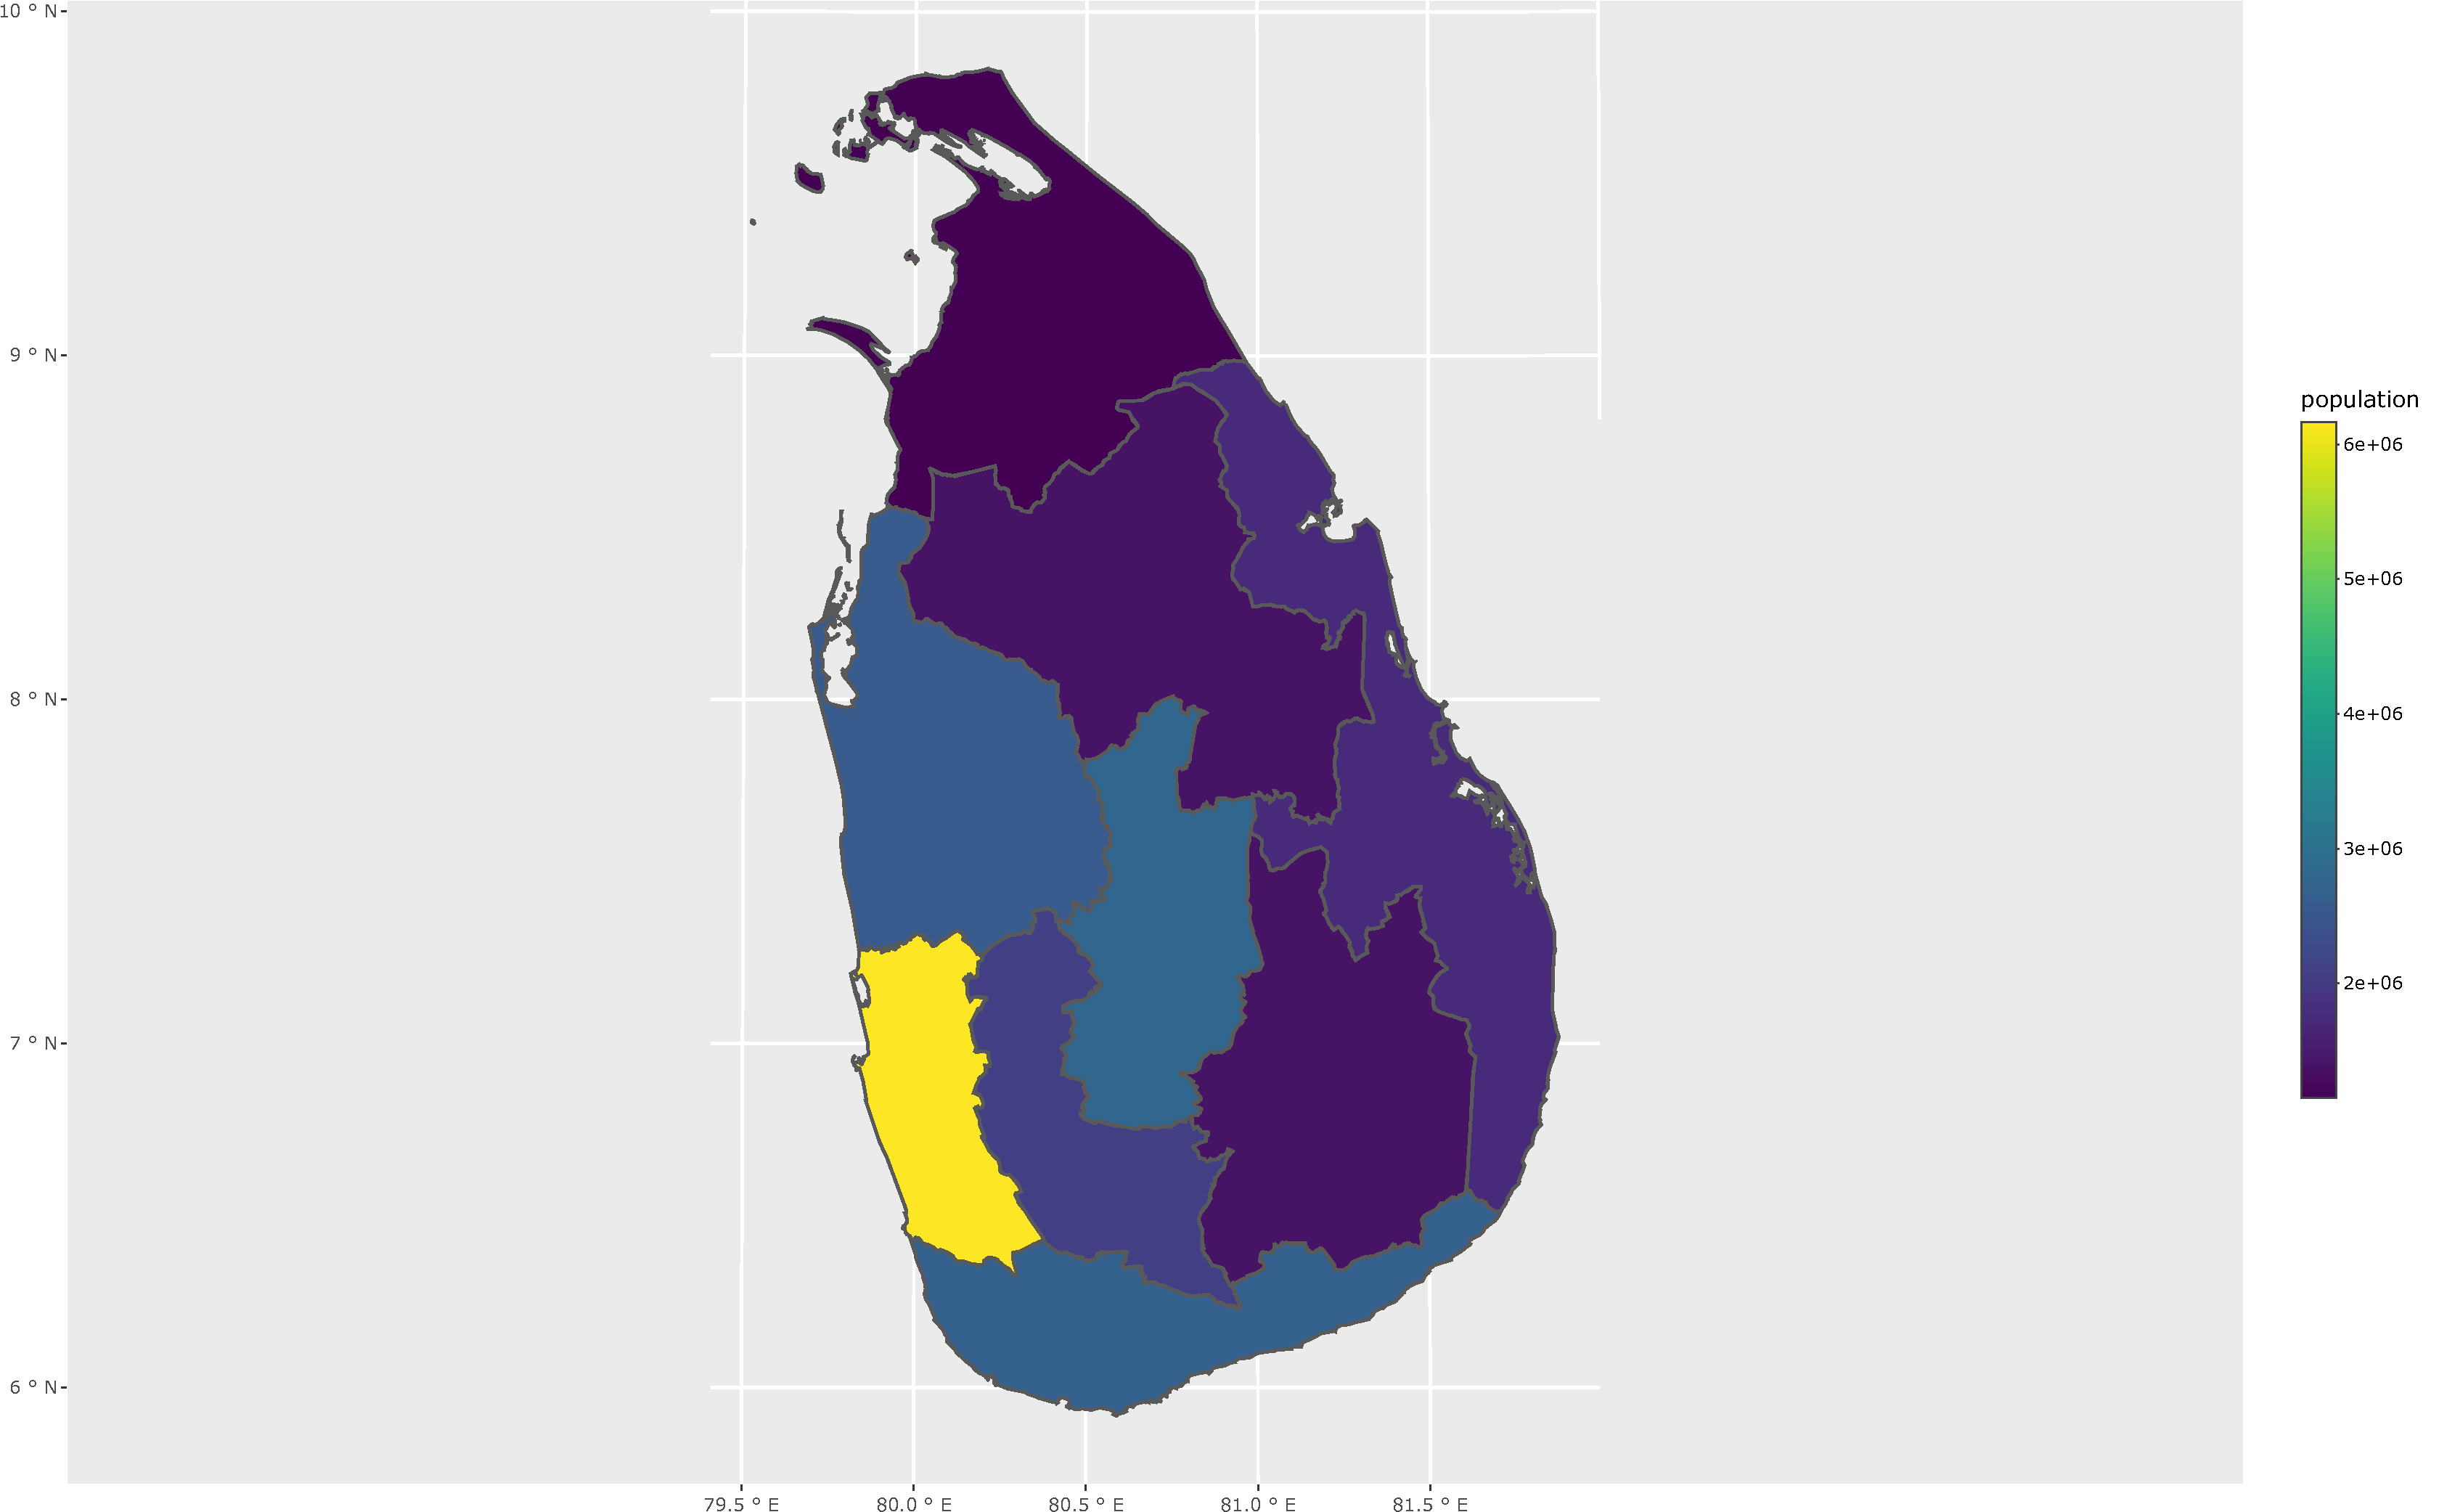
\includegraphics{chap2_files/figure-pdf/unnamed-chunk-30-1.pdf}

\hypertarget{vector-operations}{%
\section{Vector Operations}\label{vector-operations}}

To be added

\hypertarget{creating-matrix}{%
\section{Creating Matrix}\label{creating-matrix}}

\hypertarget{matrix-operations}{%
\section{Matrix Operations}\label{matrix-operations}}

\hypertarget{exercise-2}{%
\section{Exercise}\label{exercise-2}}

\begin{enumerate}
\def\labelenumi{\roman{enumi}.}
\tightlist
\item
  Write R codes to obtain following matrix outputs
\end{enumerate}

\begin{enumerate}
\def\labelenumi{\alph{enumi}.}
\tightlist
\item
\end{enumerate}

\begin{verbatim}
     [,1] [,2] [,3] [,4] [,5]
[1,]   10   30   50   70   90
[2,]   20   40   60   80  100
\end{verbatim}

\begin{enumerate}
\def\labelenumi{\alph{enumi}.}
\setcounter{enumi}{1}
\tightlist
\item
\end{enumerate}

\begin{verbatim}
     [,1] [,2] [,3] [,4] [,5]
[1,]   10   20   30   40   50
[2,]   60   70   80   90  100
\end{verbatim}

\begin{enumerate}
\def\labelenumi{\alph{enumi}.}
\setcounter{enumi}{2}
\tightlist
\item
\end{enumerate}

\begin{verbatim}
     C1 C2 C3 C4
Row1  1  6 11 16
Row2  2  7 12 17
Row3  3  8 13 18
Row4  4  9 14 19
Row5  5 10 15 20
\end{verbatim}

\begin{enumerate}
\def\labelenumi{\arabic{enumi}.}
\setcounter{enumi}{1}
\tightlist
\item
  Mr.~Perera who lives in Soratha Mawatha - Wijerama wants to sell his
  house. He wants to decide a price for his house to list it in the
  market. He believes that the size of the house is one likely
  determinant of price. He asked from 10 homes in the neighbourhood,
  ``what price should you ask for your home?'' and the house size (in
  square feet). The collected data are shown below:
\end{enumerate}

\begin{verbatim}
   size_x price_y
1    1000     810
2    1500    1210
3    2000    1450
4    2500    1610
5    3000    1690
6    3500    2010
7    4000    1490
8    4500    1690
9    5000    1890
10   5500    2410
\end{verbatim}

\begin{enumerate}
\def\labelenumi{(\alph{enumi})}
\item
  Write an R code to input \texttt{size\_x} and \texttt{price\_y} into
  two separate vectors.
\item
  Mr.~Perera wants to compute the least squares estimates of the model
  \(\hat{Y} = \hat{\beta_0} + \hat{\beta_1}X\). Write an R code to
  compute \(\hat{\beta_0}\) and \(\hat{\beta_1}\) using the matrix
  operation \(\hat{\beta} = (X^TX)^{-1}X^TY\). Do not use the built-in
  function \texttt{lm}.
\end{enumerate}

Where,

\(\hat{\beta} =\begin{pmatrix} \hat{\beta_0} \\ \hat{\beta_1} \\ \end{pmatrix}\),
\(Y = \begin{pmatrix} y_1 \\ y_2 \\ y_3 \\ . \\ . \\ . \\ y_n \end{pmatrix}\)
and
\(X = \begin{pmatrix} 1 & x_1 \\ 1 & x_2 \\ 1 & x_3 \\ . \\ . \\ . \\ 1 & x_n \end{pmatrix}\)

\hypertarget{creating-arrays}{%
\section{Creating Arrays}\label{creating-arrays}}

\hypertarget{exercise-3}{%
\section{Exercise}\label{exercise-3}}

\begin{enumerate}
\def\labelenumi{\arabic{enumi}.}
\tightlist
\item
  Create a 3D array with 3 columns, 5 rows, and 2 layers in R, and enter
  the following values into it:
\end{enumerate}

\begin{verbatim}
 [1]  1  2  3  4  5  6  7  8  9 10 11 12 13 14 15 16 17 18 19 20 21 22 23 24 25
[26] 26 27 28 29 30
\end{verbatim}

\hypertarget{creating-data-frames}{%
\section{Creating data frames}\label{creating-data-frames}}

\hypertarget{exercise-4}{%
\section{Exercise}\label{exercise-4}}

Write a code to store the following values in a dataframe.

\begin{longtable}[]{@{}rrr@{}}
\toprule\noalign{}
Girth & Height & Volume \\
\midrule\noalign{}
\endhead
\bottomrule\noalign{}
\endlastfoot
8.3 & 70 & 10.3 \\
8.6 & 65 & 10.3 \\
8.8 & 63 & 10.2 \\
10.5 & 72 & 16.4 \\
10.7 & 81 & 18.8 \\
10.8 & 83 & 19.7 \\
11.0 & 66 & 15.6 \\
11.0 & 75 & 18.2 \\
11.1 & 80 & 22.6 \\
11.2 & 75 & 19.9 \\
\end{longtable}

\hypertarget{subsetting}{%
\section{Subsetting}\label{subsetting}}

\hypertarget{exercise-5}{%
\section{Exercise}\label{exercise-5}}

This exercise is based on \texttt{mtcars} built-in-dataset in R. Write R
codes to obtain the answers for the followings.

\begin{enumerate}
\def\labelenumi{\arabic{enumi}.}
\tightlist
\item
  To obtain the help file of \texttt{mtcars}
\end{enumerate}

\begin{enumerate}
\def\labelenumi{\arabic{enumi}.}
\setcounter{enumi}{1}
\tightlist
\item
  How many cars are in the mtcars dataset?
\end{enumerate}

\begin{enumerate}
\def\labelenumi{\arabic{enumi}.}
\setcounter{enumi}{2}
\tightlist
\item
  How many variables are in the mtcars dataset?
\end{enumerate}

\begin{enumerate}
\def\labelenumi{\arabic{enumi}.}
\setcounter{enumi}{3}
\tightlist
\item
  What are the column names of the mtcars dataset?
\end{enumerate}

\begin{enumerate}
\def\labelenumi{\arabic{enumi}.}
\setcounter{enumi}{4}
\tightlist
\item
  What is the mean miles per gallon (mpg) of the cars in the dataset?
\end{enumerate}

\begin{enumerate}
\def\labelenumi{\arabic{enumi}.}
\setcounter{enumi}{5}
\tightlist
\item
  Which car has the highest horsepower (hp)?
\end{enumerate}

\begin{enumerate}
\def\labelenumi{\arabic{enumi}.}
\setcounter{enumi}{6}
\tightlist
\item
  What is the mean weight (wt) of the cars in the dataset?
\end{enumerate}

\begin{enumerate}
\def\labelenumi{\arabic{enumi}.}
\setcounter{enumi}{7}
\tightlist
\item
  How many cars have 8 cylinders (cyl)?
\end{enumerate}

\begin{enumerate}
\def\labelenumi{\arabic{enumi}.}
\setcounter{enumi}{8}
\tightlist
\item
  What is the range of displacement (disp) values in the dataset?
\end{enumerate}

\begin{enumerate}
\def\labelenumi{\arabic{enumi}.}
\setcounter{enumi}{9}
\tightlist
\item
  What is the median quarter mile time (qsec) for the cars?
\end{enumerate}

\begin{enumerate}
\def\labelenumi{\arabic{enumi}.}
\setcounter{enumi}{10}
\tightlist
\item
  How many cars have a manual transmission (am = 1)?
\end{enumerate}

\begin{enumerate}
\def\labelenumi{\arabic{enumi}.}
\setcounter{enumi}{11}
\tightlist
\item
  What is the maximum miles per gallon (mpg) in the dataset?
\end{enumerate}

\begin{enumerate}
\def\labelenumi{\arabic{enumi}.}
\setcounter{enumi}{12}
\tightlist
\item
  What is the minimum horsepower (hp) recorded in the dataset?
\end{enumerate}

\begin{enumerate}
\def\labelenumi{\arabic{enumi}.}
\setcounter{enumi}{13}
\tightlist
\item
  Which car has the lowest weight (wt)?
\end{enumerate}

\begin{enumerate}
\def\labelenumi{\arabic{enumi}.}
\setcounter{enumi}{14}
\tightlist
\item
  How many cars have 4 gears (gear)?
\end{enumerate}

\begin{enumerate}
\def\labelenumi{\arabic{enumi}.}
\setcounter{enumi}{15}
\tightlist
\item
  What is the standard deviation of the mpg variable?
\end{enumerate}

\begin{enumerate}
\def\labelenumi{\arabic{enumi}.}
\setcounter{enumi}{16}
\tightlist
\item
  What is the total number of carburetors (carb) for all cars combined?
\end{enumerate}

\begin{enumerate}
\def\labelenumi{\arabic{enumi}.}
\setcounter{enumi}{17}
\tightlist
\item
  How many cars have a quarter mile time (qsec) less than 18 seconds?
\end{enumerate}

\begin{enumerate}
\def\labelenumi{\arabic{enumi}.}
\setcounter{enumi}{18}
\tightlist
\item
  What is the mean value of the gear variable for cars with 6 cylinders
  (cyl)?
\end{enumerate}

\begin{enumerate}
\def\labelenumi{\arabic{enumi}.}
\setcounter{enumi}{19}
\tightlist
\item
  How many cars have more than 100 horsepower (hp)?
\end{enumerate}

\begin{enumerate}
\def\labelenumi{\arabic{enumi}.}
\setcounter{enumi}{20}
\tightlist
\item
  What is the correlation between horsepower (hp) and miles per gallon
  (mpg)?
\end{enumerate}

\bookmarksetup{startatroot}

\hypertarget{working-with-built-in-functions-in-r}{%
\chapter{Working with Built-in-Functions in
R}\label{working-with-built-in-functions-in-r}}

\bookmarksetup{startatroot}

\hypertarget{writing-your-own-functions}{%
\chapter{Writing Your Own Functions}\label{writing-your-own-functions}}

\bookmarksetup{startatroot}

\hypertarget{control-structures}{%
\chapter{Control Structures}\label{control-structures}}

\bookmarksetup{startatroot}

\hypertarget{introduction-to-tidyverse}{%
\chapter{Introduction to Tidyverse}\label{introduction-to-tidyverse}}

\bookmarksetup{startatroot}

\hypertarget{data-wrangling}{%
\chapter{Data Wrangling}\label{data-wrangling}}

\bookmarksetup{startatroot}

\hypertarget{data-visualisation-with-grammar-of-graphics}{%
\chapter{Data Visualisation with Grammar of
Graphics}\label{data-visualisation-with-grammar-of-graphics}}

\bookmarksetup{startatroot}

\hypertarget{reproducible-documenting-with-r}{%
\chapter{Reproducible Documenting with
R}\label{reproducible-documenting-with-r}}

\bookmarksetup{startatroot}

\hypertarget{regression-analysis}{%
\chapter{Regression Analysis}\label{regression-analysis}}

\hypertarget{introduction}{%
\section{Introduction}\label{introduction}}

\hypertarget{simple-linear-regression}{%
\section{Simple Linear Regression}\label{simple-linear-regression}}

\hypertarget{multiple-linear-regression}{%
\section{Multiple Linear Regression}\label{multiple-linear-regression}}

\hypertarget{regression-with-dummy-variables}{%
\section{Regression with Dummy
Variables}\label{regression-with-dummy-variables}}

\hypertarget{exercise-6}{%
\section{Exercise}\label{exercise-6}}

\begin{enumerate}
\def\labelenumi{\arabic{enumi}.}
\tightlist
\item
  To understand the effectiveness of marketing investments, a manager of
  a company wants to analyze the relationship between marketing
  expenditures (USD) and the number of sales. Fit a simple linear
  regression model with marketing spend as the independent variable and
  sales as the dependent variable. Interpret the outputs. Note that,
  before fitting a regression model, it is essential to conduct an
  exploratory analysis.
\end{enumerate}

\begin{tabular}{c|c}
\hline
Marketing expenditures (USD) & Number of Sales\\
\hline
100 & 522.3\\
\hline
115 & 596.2\\
\hline
120 & 617.7\\
\hline
132 & 682.3\\
\hline
144 & 740.2\\
\hline
154 & 792.5\\
\hline
158 & 806.4\\
\hline
160 & 813.5\\
\hline
170 & 871.0\\
\hline
180 & 920.6\\
\hline
181 & 927.9\\
\hline
190 & 968.5\\
\hline
200 & 1021.6\\
\hline
210 & 1068.2\\
\hline
220 & 1118.9\\
\hline
230 & 1171.2\\
\hline
240 & 1217.3\\
\hline
250 & 1272.1\\
\hline
260 & 1323.6\\
\hline
270 & 1369.6\\
\hline
\end{tabular}

2.To evaluate the association of marketing expenditures on sales, a
company manager aims to analyze the relationship between marketing
expenditures and sales across two different locations. Fit a multiple
linear regression model with marketing expenditures and location as the
independent variables and sales as the dependent variable. Interpret the
outputs. Note that, before fitting a regression model, it is essential
to conduct an exploratory analysis.

\begin{tabular}{c|c|c}
\hline
Marketing expenditures (USD) & Number of Sales & Location\\
\hline
100 & 522.3 & A\\
\hline
115 & 596.2 & A\\
\hline
120 & 617.7 & A\\
\hline
132 & 682.3 & A\\
\hline
144 & 740.2 & A\\
\hline
154 & 792.5 & A\\
\hline
158 & 806.4 & A\\
\hline
160 & 813.5 & A\\
\hline
170 & 871.0 & A\\
\hline
180 & 920.6 & A\\
\hline
181 & 927.9 & A\\
\hline
190 & 968.5 & A\\
\hline
200 & 1021.6 & A\\
\hline
210 & 1068.2 & A\\
\hline
220 & 1118.9 & A\\
\hline
230 & 1171.2 & A\\
\hline
240 & 1217.3 & A\\
\hline
250 & 1272.1 & A\\
\hline
260 & 1323.6 & A\\
\hline
270 & 1369.6 & A\\
\hline
100 & 522.3 & B\\
\hline
115 & 596.2 & B\\
\hline
120 & 617.7 & B\\
\hline
132 & 682.3 & B\\
\hline
144 & 740.2 & B\\
\hline
154 & 792.5 & B\\
\hline
158 & 806.4 & B\\
\hline
160 & 813.5 & B\\
\hline
170 & 871.0 & B\\
\hline
180 & 920.6 & B\\
\hline
181 & 927.9 & B\\
\hline
190 & 968.5 & B\\
\hline
200 & 1021.6 & B\\
\hline
210 & 1068.2 & B\\
\hline
220 & 1118.9 & B\\
\hline
230 & 1171.2 & B\\
\hline
240 & 1217.3 & B\\
\hline
250 & 1272.1 & B\\
\hline
260 & 1323.6 & B\\
\hline
270 & 1369.6 & B\\
\hline
\end{tabular}

\bookmarksetup{startatroot}

\hypertarget{summary}{%
\chapter{Summary}\label{summary}}

In summary, this book has no content whatsoever.

\begin{Shaded}
\begin{Highlighting}[]
\DecValTok{1} \SpecialCharTok{+} \DecValTok{1}
\end{Highlighting}
\end{Shaded}

\begin{verbatim}
[1] 2
\end{verbatim}

\bookmarksetup{startatroot}

\hypertarget{references}{%
\chapter*{References}\label{references}}
\addcontentsline{toc}{chapter}{References}

\markboth{References}{References}

\hypertarget{refs}{}
\begin{CSLReferences}{0}{0}
\end{CSLReferences}



\end{document}
